\documentclass[12pt]{scrbook}
\usepackage{geometry}
\usepackage{graphicx}
\usepackage{import}
\usepackage{xcolor}
\usepackage{listings}
\usepackage{caption}
\usepackage{hyperref}
\usepackage{tikz}
\usetikzlibrary{calc,positioning,shapes.geometric}

\geometry{a4paper}
\setlength{\parindent}{0pt}

%\DeclareCaptionFont{white}{\color{white}}
%DeclareCaptionFormat{listing}{\colorbox[cmyk]{0.43, 0.35, 0.35,0.01}
\DeclareCaptionFormat{listing}{\colorbox{black!15}
  {\parbox{5cm}{#1#2#3}}}
\captionsetup[lstlisting]{format=listing,
%labelfont=white,textfont=white, 
singlelinecheck=false, margin=0pt, font={bf,footnotesize}}

\begin{document}
\title{OpenPEARL - Runtime System}
\author{R. M\"uller}

\lstnewenvironment{CppCode} {
    \lstset{numbers=left,
            title={C++},
            frame=tlrb,
	    breaklines = true,
	    belowcaptionskip=4pt
    }
}%
{}%

\lstnewenvironment{PEARLCode} {
    \lstset{numbers=left,
            title={PEARL},
            frame=tlrb,
	    breaklines = true,
	    belowcaptionskip=4pt
    }
}%
{}%

\newenvironment{classSummary}%
{\vspace{3mm}\colorbox{black!15}{\parbox{5cm}{Class Summary}}\\
\begin{tabular}{|p{5cm}|p{9cm}|}
\hline
Item & Value \\
\hline}
{\hline\end{tabular}\vspace{3mm}}

\newenvironment{methodMapping}%
{\vspace{3mm}\colorbox{black!15}{\parbox{5cm}{Method Mapping}}\\
\begin{tabular}{|p{3cm}|p{4cm}|p{6.5cm}|}
\hline
Operation & Method & Remarks\\
\hline}
{\hline\end{tabular}\vspace{3mm}}

\pagestyle{myheadings}
\markboth {OpenPEARL Runtime \today} {OpenPEARL Runtime \today}

\maketitle

\tableofcontents

\chapter*{History}
The following table lists major changes of the document.

\begin{tabular}{|l|c|p{10cm}|}
\hline
date & who & change \\
\hline
29.7.2014 & rm & initial version created, some parts still missing \\
6.8.2014 & rm & wiki content moved into this paper \newline
                layout modifications\newline
                semaphore part modified\\
17.8.2014 & rm & mainly typing \\
25.8.2014 & rm & samples for WRITE and SEND added \newline
		 hyperref added\\
20.12.2014 & rm & Interrupts added \\
7.1.2015 & rm & System dation interface added \\
4.3.2015 & rm &  TaskCommon after merge of FreeRTOS and Linux \newline
and lot of minor small changes \\
28.12.2015 & rm & file system structure update \newline
                  lpc1768 timer operation added \newline
                  lpc1768 system overview cleaned \\
7.9.21016 & rm & Provider in system dations added\newline
                 Array and Struct support added\\
21.7.2017 & rm & support for simple data types reduced
                 a forwarded to the doxygen output \newline
                 Driver architecture for FreeRTOS systems added \newline
                 FatFS support for FreeRTOS added \newline
                 Porting Guide added \\
23.11.2017 & rm & some stuff moved to platform manual\\
13.12.2017 & rm & GLOBAL and IOJob Interface added \\
8.6.2018 & rm & notice about usage of thread support by C++ added in chapter
                introduction.\\
20.7.2018 & rm & Task API simplified; example code moved into doxygen \\
4.6.2019 & rm & GenericUart operation description extended \newline
                suspend and terminate during i/o operation added in FreeRTOS part\\
\hline
\end{tabular} 

\chapter{Introduction}
A PEARL program consists of several separatly compilable modules.
The interface between the modules is defined by SPC and DCL statements with the
attribute GLOBAL.
The GLOBAL statement has an optioal parameter for the module which defines the symbol.
In OpenPEARL, this parameter default to the actual module name. This suits for the specification
of SYSTEM part elements of the same module. 
The declaration of plattform dependent elements like INTERRUPTs, 
DATIONs and SIGNALs must be done in the SYSTEM-part.

For proper operation the types of the specified and declared elements must
fit. 
For system elements, we need a mechanism to obtain the type in an
extensible way. This is solved by the use of an interface definition as 
xml-file for each system element.

This tool checks all global definitions and specifications and checks for
\begin{itemize}
\item proper types, including the types of system elements
\item multiple declarations
\item missing declarations
\item unused declarations
\end{itemize}

\section{Structure}
As shown in \cite{mueller2016} the structure of operation of the \OpenPEARL{}
compilation system is like:
\newcommand*\circled[1]{\tikz[baseline=(char.base)]{
   \node[shape=circle,fill=white,draw,minimum size = 0.5cm, inner sep=2pt] (char) {#1};}}

\begin{figure}[bpht]

  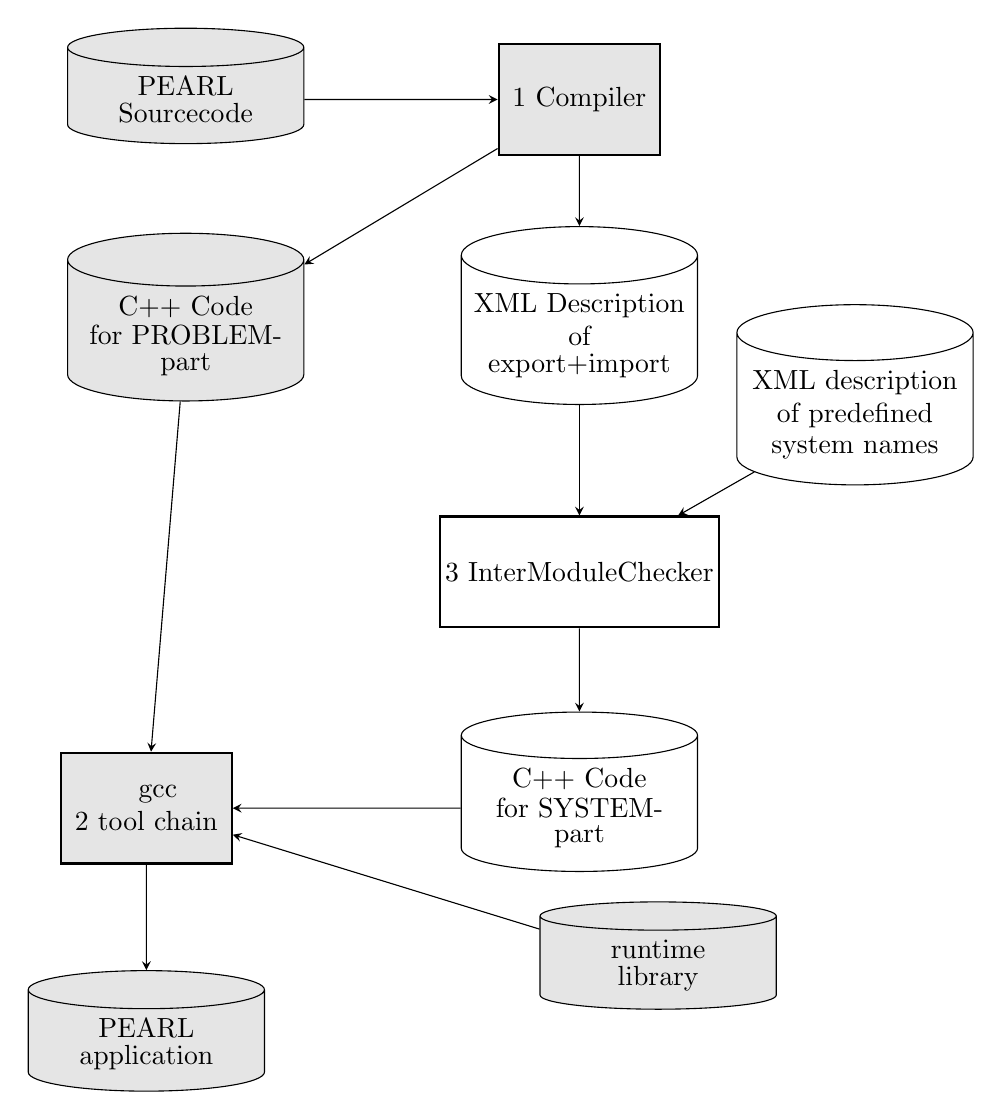
\begin{tikzpicture}[
    >=stealth,
    node distance=3.5cm,
    file/.style={
      cylinder,
      cylinder uses custom fill,
      %cylinder body fill=yellow!50,
      %cylinder end fill=yellow!50,
      shape border rotate=90,
      minimum width=3cm,
      aspect=0.25,
      draw
    },
        fileold/.style={
          cylinder,
          cylinder uses custom fill,
          cylinder body fill=gray!20,
          cylinder end fill=gray!20,
          shape border rotate=90,
          minimum width=3cm,
          aspect=0.25,
          draw
        },
    block/.style = { rectangle,
    				draw=black,
    				 thick, 
                    %fill=blue!20,
                    text centered, minimum width=5em,
                    %rounded corners,
                    inner sep = 2pt,
                    minimum height=4em },
    blockold/.style = { rectangle,
       				draw=black,
       				 thick, 
                       fill=gray!20,
                       text centered, minimum width=5em,
                       %rounded corners,
                       inner sep = 0.5em,
                       minimum height=4em }                          
  ]
    \node[fileold] (prl) at (0,10) {\shortstack{PEARL\\Sourcecode}};
    \node[blockold] (sprachumsetzer) at (5,10) {\circled{1} Compiler};
    \node[fileold,below of=prl,yshift=0.5cm] (problemcc) {\shortstack{C++ Code\\for PROBLEM-\\part}};
    \node[file,below of=sprachumsetzer,yshift=0.5cm] (modulxml) {\shortstack{XML Description
                                                            \\of \\
                                                             export+import}};
    \draw[->] (prl) -- (sprachumsetzer);
    \draw[->] (sprachumsetzer) -- (problemcc);
    \draw[->] (sprachumsetzer) -- (modulxml);

    \node[file, yshift=-1cm,right of=modulxml] (hardwarexml) {\shortstack{XML description \\of predefined\\system names}};
    \node[block, below of=modulxml,yshift=0.5cm] (imc) {\circled{3} InterModuleChecker};

    \draw [->] (modulxml) --  (imc);
    \draw [->] (hardwarexml) -- (imc);
    
    \node[file, below of=imc,yshift=0.5cm] (systemcc) {\shortstack{C++ Code\\ for SYSTEM- \\part}};
    \node[fileold, below of=systemcc, yshift=1.5cm, xshift=1cm] (runtimelib) {\shortstack{runtime\\library}};
    \node[blockold, left of=systemcc,xshift=-2cm] (gcc)
    {\circled{2}
    {\shortstack{gcc\\tool chain}}};
    \draw[->] (imc) -- (systemcc);
    \draw[->] (systemcc) -- (gcc);
    \draw[->] (runtimelib) -- (gcc);
    \draw[->] (problemcc) -- (gcc);
    
    \node[fileold, below of=gcc,yshift=0.5cm] (pearlapp) {\shortstack{PEARL\\application}};
    \draw[->] (gcc) -- (pearlapp);
  \end{tikzpicture}
\caption{Structure of the \OpenPEARL{} build system.}
\label{aufbau}
\end{figure}



The first stage compiler creates an C++-representation of the PEARL-module
together with an xml-representation of the export and import interface.

The definition of system names may be done by the user to order to supply 
additional system devices.
Each system name must be accompanied by the developer with a xml-representation
of the system element. The imc tool extracts the required information
from these xml-files and verifies a proper system configuration.

\section{Credits}
This tool  was influenced by the master thesis of 
Stephan Hertig \cite{msc_hertwig}, the semester project of
M.Bauer, T-Schaz, J.Weber, T.Welte and J.Wirth \cite{openpearlss16} and
the master thesis of M. Beyer \cite{msc_beyer}.



\chapter{Language Elements to be treated by the Compiler}
The following language elements must be treated by the compiler 
without suport by the runtime system.

\begin{description}
\item[LENGTH] of FIXED, FLOAT, BIT, CHAR must be evaluated by the 
    compiler. The runtime system expects concrete lengths for each element
\item[REF] corresponds to the definition of a pointer to the 
    element. The compiler should should instanciate an object
    the templated Ref-class. This class provides the operator* with
    a check, wether the referene ist not NIL.
    Note that REF CHARACTER works different. This type is supported by the
    runtime system.
\item[CONT] Follow a pointer (\verb|*| works on the Ref-object). 
		Only REF CHAR is supplied by the runtime system
\item[TYPE] is a type declaration. The runtime expects the primitive types.
   Perhaps the TYPE can be mapped on \verb|typedef|.
\item[INV] denotes invariant. This should be checked by the compiler internally.
    Perhaps the C++ \verb|const| may work. 
%\item[ARRAY] defines an array of elements (\verb|[]| should work)
\item[STRUCT] must be mapped to C++ \verb|struct| by the compiler 
(see section \ref{sec:struct})
\item[TYPE] defines a type  upon e.g. a struct (\verb|typedef| should work)
\item[DCL] defines a element. The compiler must instantiate an object
    of the requested type. The C++ storage class modifiers should work
    without problems.
\item[SPC] specifies an element, which is declared in another module as
  GLOBAL. The C++ \verb|extern| must be used.
\end{description}

 


\chapter{Multiple Modules and GLOBAL}

PEARL supports the separation of the application into seperate modules.
In OpenPEARL, the module name given by the \texttt{MODULE(name)} statement
defines the namespace in C++.
In order to avoid conflicts with namespaces in the standard libraries,
the supplied module name gets a prefix \texttt{pearl\_}.
All user supplied identifiers reside in the namespace of the module.

The complete runtime library uses the namespace \texttt{pearlrt}.

OpenPEARL needs some other variables for the organisation. 
They may be in the same namespace, if conflicts are avoided. This is 
achieved by prefixing all user supplied identifiers with a prefix \texttt{\_}.

\begin{PEARLCode}
MODULE(moduleA);

PROBLEM;
   DCL  a FIXED GLOBAL;
   SPC b FIXED GLOBAL (moduleB);
...
! in any PROC
   a := b;
...
\end{PEARLCode}

will produce a C++ code like:
\begin{CppCode}
#include "PearlIncludes.h"

namespace pearl_moduleA {
   pearlrt::Fixed<31> _a;
}
namespace pearl_moduleB {
   extern pearlrt::Fixed<31> _b;
}
namespace pearl_moduleA {
...
// in any PROC
   _a := moduleB::_b;
...
}
\end{CppCode}




\chapter{Signals}
\label{chapter_signals}

The signal definitions are stored in the OpenOffice document {\em Signals.ods}
for all plattforms.
The signals are objects of the class \verb|pearlrt::Signal|. 
Inducing a signal becomes mapped to a C++ throw statement.
The signal reactions are caught in a \verb|try-catch| block in procedures and
tasks, which use \verb|ON| statements of PEARL.

As shown in fig. \ref{signals_ods} the perl script
{\em GenerateSignalDefinitions.pl} creates two files
{\em Signals.hh} and {\em Signals.hcc} containing the class definitions 
and static objects declarations. 

\begin{figure}[bpht]
\begin{center}
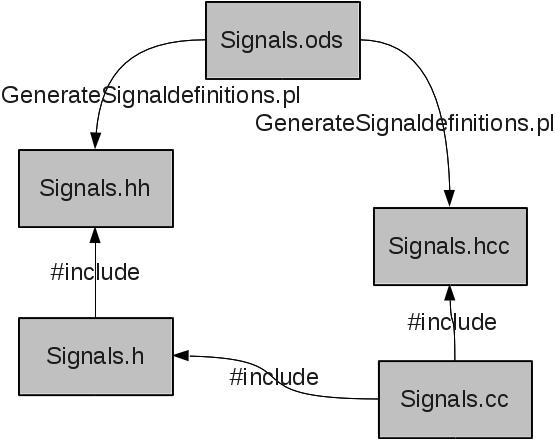
\includegraphics[width=10cm]{signals_ods.jpg}
\end{center}
\caption{Signal definitions by Spreadsheet}
\label{signals_ods}
\end{figure}

The generation is triggered by the plattform specific {\em Makefile}.
The script takes the desired target specifier(s) as command line
parameters.

\section{Signal Definition}
\label{sec_signal_definition}
The first sheet in {\em Signals.ods} contains the administrativ part.

\subsection{Grouping}
The signals are stored in groups. The definition of a group requires
an entry in the list of groups, which resides in the first sheet {\em GROUPS}
starting at line 3\footnote{This location must not be changed!}.
Each group entry consists of
\begin{description}
\item[Group name] which must have an identical name to the spreadsheet page.
   The sequence of spreadsheet pages must be identical to the sequence of
   group entries in this section.
\item[Group Number] defines the number region of the group.
    The {\em Group Number} is multiplied internally by 100.
    There may be 99 signals within each group.
\end{description}
The scripts checks for the matching of the group names and for multiple
usage of a group number.
The list of groups is terminated by an emtpy line.

\subsection{Groups}
Each group element contains the following entries:
\begin{description}
\item[GROUP INTERNAL ID] is the offset to the {\em Starting Number} of the 
   group. The id must be unique for all signals (not checked) to allow
   proper signal treatment by the runtime system.
   The {\em group internal id} 0 denotes the signal matching
   all signals defined in the group.
   The resulting signal {\em id} is created by the calculation of
   $GroupNumber \cdot 100 + GroupInternalId$
 
\item[ExceptionClass] defines the name of the C++ class, which shall be created.
   These names must by unique over all groups. This is also the name of
   the signal in the system part.
\item[ParentClass], which is used to build a C++ class hierarchy of the
    signals (C++ exceptions).
\item[System] specifies which plattform needs this signal. 
   The valid entries are defined by a drop down list. Please update the lists 
   on all sheets when a new plattform is added.
\item[Message] is the text which is sent to the standard output, when this
    signal was detected by the default signal handler.
\item[Description] contains the description of the reason for this signal
   for the external plattform signal manual. TeX syntax is allowed.
\end{description}

The scripts captures all entries of all group sheet with a matching
{\em System} entry.

\section{Decoration Scheme}
\begin{description}
\item[xxx] is the user supplied identifier for a signal
\item[theXxx] is t global identifier with the concrete signal object
\end{description}

\section{Usage in System Part}
A plattform specific signal is mapped to a user defined identifer in the 
system part. 
Each defined signal is statically instanciated to avoid
dynamic memory allocation when a exception should become thrown. 

\begin{PEARLCode}
CHAR_OVERFLOW: CharacterTooLongSignal;
\end{PEARLCode}

\begin{CppCode}
static pearlrt::Signal* _CHAR_OVERFLOW = pearlrt::theCharacterTooLongSignal;
\end{CppCode}

There is no possibility to define a signal upon its number, since this
produces lots of problems with the {\em static initialisation desaster}.
The identification of a signal at run time is done upon the signal id
which is referenced as {\em RST-value}.


\section{C++ Code for Signal Handler}
PEARL defines that a signal handler may be scheduled not inside 
a BEGIN/END-clause. The definition of a signal handler in a REPEAT block is also
prohibited. Thus we have access in the signal handler to all variables, which are defined
at the containing PROC or TASK level.
The definition of a signal handler inside of IF/THEN/ELSE-blocks is ok.

Possible reaction is a block of statements, which is executed and the
PROC is exited (the TASK teriminated) if the signal handler does not
contain a {\em GOTO-statement} defining the continuation point.
As extension to PEARL90 there a the possibility to \verb|INDUCE| the same, or another signal in OpenPEARL as signal reaction.
 
The language definition requires that a signal reaction will not triggered from inside the reation, thus a signal reaction must become disabled as soon as the
reaction becomes triggered.

The signal reactions ending with \verb|TERMINATE|, \verb|RETURN| do not require
to reenable the signal reaction, since the control flow ends with the statement.
In case of ending with an \verb|INDUCE| there might arise a problem of endless
loops between different signal reaction handlers. Thus the reaction must remain disabled when ending with \verb|INDIUCE|. 
The only case for enable a signal reaction arises with \verb|GOTO| from a signal handler into the application code.


Example:

\begin{PEARLCode}
SYSTEM;
   overfl: FixedOverFlowSignal;    
   div0:   FixedDivideByZeroSignal;
   arith:  ArithmeticSignal;

 PROBLEM;
   SPC overfl SIGNAL;
   SPC div0   SIGNAL;
   SPC arith  SIGNAL;

   X: PROC (p FIXED) 
      DCL k FIXED(15);

      k := 2;

restart: 
      ! signal action #1
      ON overfl BEGIN
         PUT 'PROC X: Arithmetic error (returning)' TO console BY A, SKIP;
         RETURN;
      END;

      ! signal action #2
      IF ( p == 1) THEN
         ON overfl BEGIN
            PUT 'PROC X: Overflow occured (terminating)' TO console BY A, SKIP;
            TERMINATE;     
         END;
      FIN;
      
      IF ( p > 5) THEN
      ! signal action #3
        ON overfl BEGIN
           PUT 'PROC X: Overflow occured (returning)' TO console BY A, SKIP;
           RETURN;
        END;
      FIN;

      ! signal action #4
      ON div0 BEGIN 
          PUT 'Divide by zero (restarting)' TO console BY A, SKIP;
          IF ( p ==  6) THEN
             GOTO EXIT;
          FIN;
          IF ( p = 11) THEN
              k:= 11//(k-k);   ! produce new div0 which is not caught again
          FIN;
          p := 6;
          GOTO RESTART;
      END;
      
      IF p == 11 THEN
          k := 10 // (k-k);  ! force 'div by 0'
      FIN;

      FOR i TO 100 REPEAT
        k := k * k;
      END;
exit:
  END;
\end{PEARLCode}

There are four signal handler defined in the procedure.
The \verb|Arithmetic| signal covers also the \verb|FixedOverFlowSignal|
and \verb|FixedDivideByZeroSignal| and some other error situations 
with arithmetics.

Since there are signals handler defined in the procedure,
the body is placed in a try-catch-block.
The catch block checks, whether the current signal matches 
on of the scheduled signal actions.

\begin{CppCode}
// system part
extern pearlrt::Signal *_overfl;
extern pearlrt::Signal * _div0;
extern pearlrt::Signal * _arith;

// problem part
SPCTASK(TASK1);

void _x(pearlrt::Task * me, pearlrt::Fixed<15> p) {
   pearlrt::Fixed<15> _k;

   //[ generated from ON statements in PROC
   pearlrt::SignalAction sigActions[5];
   pearlrt::ScheduledSignalActions scheduledSignalActions(5, sigActions);

    tryAgain:
    try {
       switch (indexOfSignalAction) {
          case -1: break;

       case 1: // first signal reaction
         ...
         break;

       } // end of switch
 
       // PROC or TASK body with schedudling of signal reactions
       ...  // normal code until first ON
      sigActions[1-1].setSignal(_artith);
      ...
      // 2nd ON
      sigActions[2-1].setSignal(_artith);
      ...
   } catch(pearlrt::Signal & s) {
       indexOfSignalAction = 
		scheduledSignalActions.getActionIndexAndSetRstAndDisableHandler(&s);
       if (indexOfSignalAction == 0) {
          // no handler found
          throw;
       }
       goto tryAgain; // signal handler found
    }
    // END OF SIGNAL FRAME
}  and of PROC or TASK
\end{CppCode}


Remarks:
\begin{description}
\item[disable signal handler] is done if the signal handler becomes
   active. Enabling is only necessray, if the handler is exited 
   with a GOTO statement, which requires a modified C++ code generation,
   when a GOTO statement leaves the range of a signal handler.
\item[sigActions] must be of type auto to provide task and procedure specific 
   signal reactions.
\end{description}

\section{C++ Code for Signal Handler with RST-Tag}
When a RST-element is specified in the ON-statement, the current
RST-value must be read into the given variable.

\begin{PEARLCode}
DCL Errorcode FIXED(15);
...
   ! version 1  ON statement in proc/task
   ON overfl RST(Errorcode): BEGIN .... END;

   ! version 2  ON statement in proc/task
   ON overfl RST(Errorcode);
\end{PEARLCode}

Version 1 is treated inside the function \verb|ScheduledSignalReactions::getActionIndexAndSetRstAndDisableHandler(Signal*s);|

Version 2 require that each statement in the task or procedure body ---
including the signal reactions --- becomes wrapped with a try catch block like:

\begin{CppCode}
    try {
       _x = CONST_FIXED_P_10_4;
    } catch (pearlrt::Signal & s) {
       scheduledSignalActions.setErrorOrThrow(&s);
    }
\end{CppCode}

This wrapping could be omitted for statements which do not 
throw a signal exception. This is part of a future check in the compiler.


\section{Induce}
The statement {\em INDUCE} simulates a signal and causes the trigger 
of the scheduled reaction.
Note that OpenPEARL forbids an induce statement with a RST-value.


\begin{PEARLCode}
INDUCE div_0;
\end{PEARLCode}

\begin{CppCode}
throw *_div_0;
\end{CppCode}

\section{Groups of Signals and Delegation of Signals to invoking Procedures and Task}


\begin{PEARLCode}
SYSTEM;
   TaskRunningSignal: TaskRunningSignal; ! number 102
   Arithmetic: ArithmethicSignal;        ! number 200

PROBLEM;
   SPC TaskRunningSignal SIGNAL;
   SPC Arithmetic SIGNAL;
   DCL Errorcode Fixed;
   DCL counter FIXED INIT(0);

Prog: TASK MAIN;
    ALL 1 SEC ACTIVATE Demo;
END;

Demo: TASK; 
   counter := counter + 1;

   ON TaskRunningSignal RST(ErrorCode)
	PUT 'TaskSignal occured with RST=', ErrorCode TO console BY A,F,SKIP;
   ON Arithimetic RST(ErrorCode)
	PUT 'Arithmetic problem occured with RST=', ErrorCode TO console BY A,F,SKIP;

   Test;
END;

Test: PROC;
   DCL k FIXED(15) INIT(2);

   CASE counter
   ALT /* 1 */ INDUCE TaskRunningSignal;
   ALT /* 2 */ k = k//(k-k);   ! produce divide by zero
   ALT /* 3 */ REPEAT  
	  	k = k * 2;  ! procuces FixedOverflowSignal
	       END;
   FIN;
END;
\end{PEARLCode}

This program will produce the output
\begin{verbatim}
TaskSignal occured with RST=200
Arithmetic problem occured with RST=102
Arithmetic problem occured with RST=103
\end{verbatim}

Sample C++ Code:
\begin{CppCode}
c++ code missing
\end{CppCode}

\chapter{Simple Data Types}
PEARL defines the data types FIXED, FLOAT, BIT, CHARACTER, REF CHARACTER,
DURATION and CLOCK.

Specific for PEARL is the signal mechanism. It is expected that
each operation induces a signal (in C++ exception) if the operator
does no finish successfully. C++ does not provide this feature.

For each data type a separate class provides the required operations.
FIXED, FLOAT, BIT and CHARACTER may be defined in PEARL with a length
attribute. This is mapped to C++-templates.

For details about ctor parameters and member functions please check the
doxygen documentation, which can be created for a specific plattform
by \verb|make doc| in the corresponding directory.

The classes for the simple data types are named as:

\begin{tabular}{|l|l|l|}
\hline\\
PEARL name & class name & remarks\\
\hline
FIXED & Fixed & templated with the length\\
FLOAT & Float & templated with the length\\
BIT & BitString & templated with the length\\
CHAR & Character & templated with the length\\
REF CHAR & RefCharacter & \\
DURATION & Duration & \\
CLOCK & Clock & \\
\hline
\end{tabular}

\if0
\section{Fixed}
The class {\em Fixed63} provides save operations on fixed values 
with 63 bits plus sign. This development of this class was influenced by
the header SafeInt.hxx, which is provided with the MSPL license.
This class is used internally for the implementation of fixed values
with individual lengths.

The application specific versions of  the type fixed are realized with the 
C++ template mechanism in {\em Fixed.h},
 requiring the number of mantissa bits as template parameter. 
All lengths from 1 to 63 are suported.
The operations are mapped to the usual C++-operators.  
For PEARL-specific operations member functions are supplied.

All operations, which produce numerical {\em overflow}, {\em underflow}
 or {\em divide by zero}  throw an exception.

\begin{classSummary}
 Class & \verb|Fixed<int S>| \\
 Specification & Fixed.h \\
 Implementation & - \\
 \verb|size(Fixed<7>)| &   1 byte \\
 \verb|size(Fixed<15>)| & 2 bytes \\
 \verb|size(Fixed<31>)| & 4 bytes \\
 \verb|size(Fixed<63>)| & 8 byte  \\
\end{classSummary}


\begin{methodMapping}
  \verb|+| (monadic)      &        & to be treated by the compiler \\
  \verb|-| (monadic)    & \verb|operator-()| &  \\
 \verb|ABS|            & \verb|absVal()|  &  \\
 \verb|SIGN|           & \verb|sign()|  & \\
 \verb|TOBIT|          & \verb|BitString| &
                    realized as Ctor in BitString 
                     with the component '.x' of the FIXED variable \\
 \verb|TOCHAR|         & \verb|toChar()|  & realized in Character.h \\
  \verb|+| (dyadic)     & \verb|operator+(rhs)| & \\
  \verb|-| (dyadic)     & \verb|operator-(rhs)| & \\
  \verb|*| (dyadic)     & \verb|operator*(rhs)| & \\
  \verb|//| (dyadic)   & \verb|operator/(rhs)| & \\
  \verb|REM| (dyadic)   & \verb|operator%(rhs)| & \\
  \verb|**| (dyadic)    & \verb|pow(rhs)|    & rhs is the exponent \\
  \verb|<|          & \verb|operator<(rhs)|  & \\
  \verb|>|           & \verb|operator>(rhs)|  & \\
  \verb|<=|         & \verb|operator<=(rhs)| & \\      
  \verb|>=|         & \verb|operator>=(rhs)| & \\   
  \verb|==|         & \verb|operator==(rhs)| &   \\
  \verb|/=|        & \verb|operator!=(rhs)|  &   \\
  FIT               & \verb|fit(rhs)|    & rhs defines target size \\
\end{methodMapping}

\paragraph{Remarks:}
\begin{itemize}
\item If no preset value is specified, the variable is initialized with 0.
\item There is no default length in the runtime system.
\item C++ literals correspond usually to 32 bit integers. 
If we need longer constants the postfix \verb|LL| must be added by
the compiler to enforce 64-bit integers.
\end{itemize}

\begin{PEARLCode}
DCL x FIXED(31) INIT(15); 
DCL y FIXED(33) INIT(16); 
DCL z FIXED INIT(17); 
DCL z1 FIXED;
DCL longFixed Fixed(53) INIT(123456789012); 
z := x + y;
x := z FIT x;
x := z ** y;
\end{PEARLCode}


\begin{CppCode}
Fixed<31> x(15);
Fixed<33> y(16);
Fixed<31> z(17);
Fixed<31> z1;
Fixed<53> longFixed(123456789012LL); 
z = x + y;
x = z.fit(x);
x = z.pow(y);
\end{CppCode}


\section{Float}

The type FLOAT is provided by templates with the lengths 24 and 53 bit
mantissa precission, both with the hidden one presentation.
These lengths are defined by the IEEE754 
standard types single and double.

New float variables are initialized with {\em NaN}, which is defined
as \verb|NAN| in the {\em math.h} GNU-library if IEEE754 is
available on the current system. This preset avoids problems with 
uninitialized float values in calculations.

Each operation (except assignment and comparison) contain checks
for unexpected results. A result of {\em NaN} or {\em INF} causes the signals
{\em FloatIsNaNSignal} or {\em FloatIsINFSignal} to be emitted.

The operations are mapped to the usual C++-operators.  
For PEARL-specific operations member functions are supplied.

\begin{classSummary}
 Class & \verb|Float<24>| and \verb|Float<53>|\\
 Specification & Float.h \\
 Implementation & - \\
 \verb|size(Float<24>)| &   4 byte \\
 \verb|size(Float<53>)| & 8 bytes \\
\end{classSummary}


\begin{methodMapping}
  \verb|+| (monadic)      &        & to be treated by the compiler \\
  \verb|-| (monadic)    & \verb|operator-()| &  \\
 \verb|ABS|            & \verb|abs()|  &   \\
 \verb|SIGN|           & \verb|sign()|   &  \\
 \verb|ENTIER|          & \verb|entier()| & \\
 \verb|ROUND|          & \verb|round()| & \\
  \verb|+| (dyadic)     & \verb|operator+(rhs)| & rhs may be Fixed or Float\\
  \verb|-| (dyadic)     & \verb|operator-(rhs)| & rhs may be Fixed or Float\\
  \verb|*| (dyadic)     & \verb|operator*(rhs)| & rhs may be Fixed or Float\\
  \verb|/| (dyadic)   & \verb|operator/(rhs)| & rhs may be Fixed or Float\\
  \verb|**| (dyadic)    & \verb|pow(rhs)|    &
                rhs is the exponent with type \verb|Fixed<S>| \\
  \verb|<|          & \verb|operator<(rhs)|  & rhs may be Fixed or Float\\
  \verb|>|           & \verb|operator>(rhs)|  & rhs may be Fixed or Float \\
  \verb|<=|         & \verb|operator<=(rhs)| & rhs may be Fixed or Float \\     
  \verb|>=|         & \verb|operator>=(rhs)| & rhs may be Fixed or Float \\   
  \verb|==|         & \verb|operator==(rhs)| & rhs may be Fixed or Float \\
  \verb|/=|        & \verb|operator!=(rhs)|  & rhs may be Fixed or Float   \\
  FIT               & \verb|fit(rhs)|    & rhs defines target size \\
SIN			& \verb|sin()|	& rhs must be Float \\ 
COS			& \verb|cos()|	& rhs must be Float \\ 
TAN			& \verb|tan()|	& rhs must be Float \\ 
ATAN			& \verb|atan()|	& rhs must be Float \\ 
TANH			& \verb|tanh()|	& rhs must be Float \\ 
EXP			& \verb|exp()|	& rhs must be Float \\ 
LN			& \verb|ln()|	& rhs must be Float \\ 
SQRT			& \verb|sqrt()|	& rhs must be Float \\ 
\end{methodMapping}

\paragraph{Remarks:}
\begin{itemize}
\item There is no default length in the runtime system.
\item C++ literals are passed as {\em double} to ctor.
\item mixed operations with Fixed and Float are treated b non member methods
\item sin, cos, ... with fixed is not supported yet; this must be 
   treated by the compiler with the semantic analysis by automatic
   type conversion towards Float.
\item entier and round behavior must be compared with existing implementations; 
    this implementation behaves like:
    
    \begin{tabular}{c||c|c|c|c|c|c}
     x &         10.5 & 10.4 & 10.0 & -10.0 & -10.4 & -10.5 \\
     \hline
     entier(x) & 10 & 10& 10& -10& -11 & -11 \\
     \hline
     round(x) & 11& 10& 10& -10& -10& -11 \\
   \end{tabular} 
\end{itemize}

\begin{PEARLCode}
DCL x FLOAT(24) INIT(1.5); 
DCL y FLOAT(53) INIT(1.6); 
DCL z FLOAT INIT(1.7); 
DCL z1 FIXED(31);
y := x + y;
x := z FIT x;
x := z ** y;
z := SIN(y);
z := SIN(x+y);
\end{PEARLCode}


\begin{CppCode}
Float<24> x(1.5);
Float<53> y(1.6);
Float<53> z(1.7);
Float<31> z1;
y = x + y;
x = z.fit(x);
x = z.pow(y);
z = y.sin();
z = (x+y).sin();
\end{CppCode}


\section{Bit}
The type BIT is supported by the templated class {\em BitString}.
The name was choosen to make clear that there may be  more than one bit
in variable of this type.
The internal data type is used according the length of the BitString. 
The smallest possible native data size is used (1,2,4 or 8 bytes).

The supported sizes are 1 to 64.

The alignment of the bits inside the BitString is left adjusted. 
This means that the most significant bits are used. This was choosen due to 
the definition of operations of BitStrings with differnt lengths.

Member functions are supplied for the PEARL operations. 

Bit constants define their length intrinsic. All given digits are 
considered to be part of the bit constant. E.g.

\begin{tabular}{|r|c|}
\hline
BIT constant & Type \\
\hline
'1'B & BIT(1) \\
'1'B2 & BIT(2) \\
'1'B3 & BIT(3) \\
'1'B4 & BIT(4) \\
'01'B4 & BIT(8) \\
\hline
\end{tabular}

\begin{classSummary}
 Class & \verb|BitString<int len>| \\
 Specification & BitString.h \\
 Implementation & - \\
 \verb|size(BitString<8>|) & 1 byte \\
 \verb|size(BitString<16>|) & 2 bytes \\
 \verb|size(BitString<32>)| & 4 bytes \\
 \verb|size(BitString<64>)| & 8 byte  \\
\end{classSummary}

\begin{methodMapping}
  \verb|NOT|       & \verb|bitNot()| &  \\
  \verb|TOFIXED|   & \verb|toFixed()| &  \\
  \verb|==|        & \verb|operator==(rhs)|   &  \\
  \verb|/=|        & \verb|operator!=(rhs)|   & \\
  \verb|AND|       & \verb|bitAnd(rhs)|   & \\
  \verb|OR|       & \verb|bitOr(rhs)|   & \\
  \verb|EXOR|     & \verb|bitXor(rhs)|    & \\
  \verb|><| (CAT) & \verb|bitCat(rhs)|    & \\
  \verb|<>| (CSHIFT) & \verb|bitCshift(rhs)| & \\
  \verb|SHIFT|       & \verb|bitShift(rhs)|  & \\
  \verb|.BIT(x)|     & \verb|getBit(...)|  & 
				{\em on right hand side of the expression}\\
  \verb|.BIT(x)|    & \verb|setBit(...)|  & 
				{\em on left hand side of the expression}\\
  \verb|.BIT(x,y)|  & \verb|getSlice(...)| & 
				{\em on right hand side of the expression}\\
  \verb|.BIT(x,y)|   & \verb|setSlice(...)| & 
				{\em on left hand side of the expression}\\
\end{methodMapping}

The slice operations \verb|.BIT(...)| may be used in PEARL 
on the left hand side and the right hand side of the expression.
 

\paragraph{Remarks:}
\begin{itemize}
\item The preset value is passed to the ctor as integer type. The
   radix evaluation must be done by the compiler.
\item The passed integer is shifted internally by the number of not used 
   bits in the used native data type to the left side. This results
   in the proper interal alignment.
\item If no preset value is specified, the variable is initialized with 0.
\item There is no default length in the runtime system.
\item the method names like {\em bitAnd} were choosen since {\em and} 
is a reserved keyword in C for computer systems without \& character
\item C++ literals correspond usually to 32 bit integers. 
If we need longer constants the postfix \verb|LL| must be added by
the compiler to enforce 64-bit integers.
\item The initialising constant is of type int and right adjusted!
\item {\em getSlice} and {\em setSlice} take the start index and a 
    {\em BitString} defining the length and/or value as parameter.
\end{itemize}

Sample Code:
\begin{PEARLCode}
DCL x BIT(4) INIT ('1'B4);
DCL y BIT(4);
DCL z BIT(3);
DCL c BIT(8);
DCL f FIXED(3) INIT(2);
y := '01'B1;  // implicit conversion BIT(2) -> BIT(4)
y := x CSHIFT 1;
z := y AND x;
c := x CAT y;
y := TOBIT f;
f := TOFIXED y;
z.BIT(2,2)  := c.BIT(1,2);
\end{PEARLCode}

\begin{CppCode}
BitString<4> x4(1);
BitString<4> y;
Fixed<3> f(2);
y = (pearlrt::BitString<2>)(1);
y = x.bitCshift(1);
z = y.bitAnd(x);
c = x.bitCat(y);
y = BitString<4>(f.x);
f = y.toFixed();
z.setSlice(2,c.getSlice(1,BitString<2>dummy));
\end{CppCode}

\section{CHARACTER}
The data type CHARACTER in PEARL has a definite and fixed length.
The templated class {\em Character} provides the storage allocation
and necessary methods for this data type.
All operations check for range overflows and throw exceptions in case of
range violation.

The language report states at one location that the length is of type FIXED(15).
Therefore the supported lengths are 1 to 32787.

The preset of a character variable may be set as C-string constant.

\begin{classSummary}
 Class & \verb|Character<size_t len>| \\
 Specification & Character.h  \\
 Implementation  &  Character.cc \\
 size   &  1 byte per Character \\
 max length & 32767  \\
\end{classSummary}

\begin{methodMapping}
  \verb|UPB|      & \verb|upb()|    &  {\em returns size\_t}\\
  \verb|TOFIXED| & \verb|toFixed()| &     \\ 
  \verb|<|       & \verb|operator<()| &  \\
  \verb|>|       & \verb|operator>()| &  \\
  \verb|<=|      & \verb|operator<=()| & \\
  \verb|>=|      & \verb|operator>=()| & \\
  \verb|==|      & \verb|operator==()| & \\
  \verb|/=|      & \verb|operator!=()| & \\
  \verb|><| (CAT) & \verb|catChar()| & {\em see note below} \\
  \verb|.CHAR(x)| & \verb|setCharAt(..)|&  
				on left hand side in expression
				{\em see note below}\\
  \verb|.CHAR(x)| & \verb|getCharAt(..)| & 
				on right hand side in expression
				{\em see note below}\\
  \verb|.CHAR(x,y)| & \verb|setCharSlice()| & 
				on left hand side in expression
				{\em see note below}\\
  \verb|.CHAR(x,y)| & \verb|getCharSlice()| &
				on right hand side in expression
				{\em see note below}\\
\end{methodMapping}
The slice operations \verb|.CHAR(...)| may be used in PEARL 
on the left hand side and the right hand side of the expression.

Remarks:
\begin{itemize}
\item The slice operations are defined with a different interface than 
   BitString. This was choosen to avoid character copies.
\item the setSliceChar and getSliceChar methods take as $4^{th}$ element
a Character value defining the retrieved/new data
 from/for the container Char-value
\end{itemize}

\begin{PEARLCode}
DCL x CHARACTER(5) INIT ('PEARL');
DCL y CHARACTER(4);
y := x.CHAR(2,5);
x.CHAR(2,5) := y;
\end{PEARLCode}
\begin{CppCode}
Character<5> x("PEARL");
Character<4> y;
getSliceChar(x, 2, 5, y);
setSliceChar(x, 2, 5, y);
\end{CppCode}


\section{REF CHARACTER}
The type REF CHARACTER allows character string with variable length.
A REF CHARACTER needs a normal CHARACTER variable as working storage.
It contains an additional value to maintain the current used length.

The class {\em RefCharacter} provides the necessary operations.

\begin{classSummary}
Class & RefCharacter  \\
 Specification & RefChar.h  \\
 Implementation & RefChar.cc \\
 size   &  12 byte \\
\end{classSummary}

\begin{methodMapping}
  \verb|:=|     & \verb|setWork()|    & REF CHAR := CHAR(x) \\
  \verb|CONT|   & \verb|\verb|store()|    & CHAR := CONT REF CHAR(x) \\
\end{methodMapping}

The content based operations like comparison are done upon the
CHARACTER-type.


\begin{PEARLCode}
DCL wrk CHARACTER(100);
DCL result CHARACTER(50);
DCL rc REF CHAR();
rc := wrk;
CONT rc := 'Hallo';
CONT rc := CONT rc CAT ' Welt.';
result := CONT rc;
\end{PEARLCode}

\begin{CppCode}
Character<100> wrk;
Character<50> result;
RefCharacter rc;
rc.setWork(wrk);
rc.clear();
Character<5> hello((char*)"Hallo");
rc.add(hello);
Character<6> welt((char*)" Welt.");
rc.add(welt);
rc.store(result);
\end{CppCode}

\section{DURATION}
The values of type DURATION are managed by the class {\em Duration}.
The values are stored in a 64 bit integer ({\em Fixed63}).
The base unit is $1 \mu s$.
The range of 64 bit allows durations up to $\approx 100 days$.

All calculations on durations are done within the full possible range.
Thus values larger than 24 hours may occur.
Even negativ values are possible.

The mapping of duration values to the C++ types is done via the type
\verb|double| giving the duration in seconds.

Operations are defined as required by the language to mix DURATION, CLOCK, 
   FIXED and FLOAT.

\paragraph{Notes:}
\begin{itemize}
\item The division Duration / Duration delivers a \verb|Float<24>|, 
   which may be assigned to larger Float type
\item The division Duration/Float is realized as template for 
   all Float-lengths 
\end{itemize}

\begin{classSummary}
 Class & Duration \\
 Specification & Duration.h \\
 Implementation & Duration.cc \\
 size   &  8 bytes \\
\end{classSummary}


\begin{methodMapping}
  \verb|+| (monadic)  &        & to be treated by the compiler \\
  \verb|-| (monadic)  & \verb|operator-()|  & \\
  \verb|ABS|          & \verb|abs()|  & \\
  \verb|SIGN|         & \verb|sign()|  & \\
  \verb|+| (dyadic)   & \verb|operator+(rhs)| & duration+duration \\
  \verb|-| (dyadic)   & \verb|operator-(rhs)| & duration-duration \\
  \verb|*| (dyadic)   & \verb|operator*(rhs)| & duration*\verb|Float<S>| \\
  \verb|/| (dyadic)   & \verb|operator/(rhs)| & duration/duration returns
        \verb|Float<24>| \\
  \verb|/| (dyadic)   & \verb|operator/(rhs)| & duration/\verb|Float<S>| \\
  \verb|<|            & \verb|operator<(rhs)|& \\
  \verb|>|            & \verb|operator>(rhs)| &  \\
  \verb|<=|           & \verb|operator<=(rhs)|& \\
  \verb|>=|           & \verb|operator>=(rhs)| & \\
  \verb|==|           & \verb|operator==(rhs)| & \\
  \verb|/=|           & \verb|operator!=(rhs)| & \\
\end{methodMapping}

\begin{PEARLCode}
DCL minute DURATION INIT(1 MIN);
DCL d1 DURATION INIT(1 HRS 3 MIN 3.1415 SEC);
DCL d2 DURATION INIT(0.001415 SEC);
d2 := d1 + minute;
d2 := d1 + minute / 60.0;
\end{PEARLCode}
\begin{CppCode}
Duration minute(60.0);
Duration d1(3783.1415);
Duration d2(0.001415);
d2 = d1 + minute;
d2 = d1 + minute / (Float<24>)(60);
\end{CppCode}

\section{CLOCK}
The values of type CLOCK are managed by the class {\em Clock}.
The values are stored in a 64 bit integer ({\em Fixed63}).
The base unit is $1 \mu s$.

All calculations on clock values are done within the
period of 1 day.

The mapping of duration values to the C++ types is done via the type
\verb|double| giving the duration in seconds.

Operations are defined as required by the language to mix DURATION and CLOCK. 

The specification requires a procedure \verb|NOW| which delivers the current
time as \verb|CLOCK|-value. This routine is plattform specific.


\begin{classSummary}
 Class & Clock  \\
 Specification & Clock.h  \\
 Implementation &  Clock.cc \\
 size   &  8 byte \\
\end{classSummary}


\begin{methodMapping}
  \verb|+| (dyadic) & \verb|operator+(rhs)| & Clock + Duration \\
  \verb|-| (dyadic) & \verb|operator-(rhs)| & Clock-Duration and Clock-Clock \\
  \verb|<|          & \verb|operator<(rhs)| &
                    {\em returns bool } \\
  \verb|>|          & \verb|operator>(rhs)| & 
                    {\em returns bool } \\
  \verb|<=|         & \verb|operator<=(rhs)| &
                    {\em returns bool } \\
  \verb|>=|         & \verb|operator>=(rhs)| &
                    {\em returns bool } \\
  \verb|==|         & \verb|operator==(rhs)| & 
                    {\em returns bool } \\
  \verb|/=|         & \verb|operator!=(rhs)| & 
                    {\em returns bool } \\
  \verb|NOW|        & \verb|Clock::now()| & this method is plattform specific\\
\end{methodMapping}

Remarks:
\begin{itemize}
\item the arithmetic operations are defined for also for
   mixed Duration and Clock parameters
\end{itemize}


\begin{PEARLCode}
DCL start CLOCK(11:30);
DCL current CLOCK;
DCL diff DURATION;
current := NOW;
diff := current - start;
\end{PEARLCode}

\begin{CppCode}
Clock start(41400.0);
Clock current;
Duration diff;
current = now();
diff = current - start;
\end{CppCode}
\fi


\chapter{Struct, Type and Arrays}

\section{Struct}
\label{sec:struct}

PEARL structs may be mapped to C++ structs.
The C++ operators like \verb|=| (assignment), \verb|.| (dot) and 
\verb|->| (follow) will work.

One problem arises when structs are multiply defined
in PEARL. All struct with the same internal structures as
taken to be identical. C and C++ structs as not compatible
if multiply defined.

The struct statement should be mapped to a named C++ struct and the identifier
of the struct is derived from the struct components.
The C++ standard states that a C++ compiler should support at least 1024
characters for identifiers. The g++ has no limit for the length of identifiers.

Each possible data type for a struct component is mapped to a letter.
The length has a maximum length of 64 for FIXED, FLOAT and BIT. CHAR
variables may have a length of up to 32767 characters.
 C++ provides only 63 different
 characters for the use in identifiers. So we use 1-5 digits
for the length.

If the component is an array, the number of dimensions and the
 limits are
passed as \verb|_| (underscore) separated list of decimal integers
to the type.

Mapping of data types to letters:

\begin{tabular}{|l|c|c|}
\hline
Datatype & letter & REF \\
\hline
FIXED & A &a\\
FLOAT & B &b\\
BIT  & C &c\\
CHARACTER & D &d \\
CLOCK  & E &e \\
DURATION & F&f \\
TASK & & g \\
PROC  & & h \\
SEMA & I & i \\
BOLT & J & j \\
\hline
STRUCT & S &s\\
\hline
\end{tabular}

\paragraph{Note:} Semaphores and Bolts variables are not allowed in structs,
but the encoding mapping is also used for the inter module checker.


Structs are mapped to the key 'S' followed by an integer
indicating the length of the struct components.
E.g. 

Example:
\begin{PEARLCode}
... STRUCT [ 
    x FIXED(15);
    y FLOAT(53);
    ]
...
\end{PEARLCode}

The component x ist translated into A15 and y into B53.
The struct consists of these two elements with a length of
the type string of 3 digits each. Thus the content
of the struct is described by the string "'A15B53"'.
This is prefixed with "'S"' and the length of the component
descriptor leading to S6A15B53.

\begin{CppCode}
struct S6A15B53 {
   pearlrt::Fixed<15> _x;
   pearlrt::Float<53> _y;
};
\end{CppCode}

In case of combination of arrays in structs and array of structs we get:

\begin{PEARLCode}
DCL x STRUCT [
   a FIXED(7);
   b(1:3,3:10) FLOAT(24);
   c(2) STRUCT [
     c1(19) FIXED(15);
     c2 BIT(5);
     ];
  ];
\end{PEARLCode}

The name of the struct results into: 

$S37\underbrace{\underbrace{A7}_{FIXED(7)}}_{a}\underbrace{\underbrace{B24}_{Float(24)}\underbrace{\_2\_1\_3\_3\_10}_{(1:3,3:10)}}_{b(1:3,3:10)}\underbrace{\underbrace{S12\underbrace{A15\_1\_1\_19}_{c1(19) FIXED(15)}\underbrace{C5}_{c2 BIT(5)}}_{STRUCT ..}\underbrace{\_1\_1\_2}_{(2)}}_{c(2)}$


\begin{CppCode}
struct S37A7B24_2_1_3_3_10S12A15_1_1_19C5_1_1_2 {
   pearlrt::Fixed<7> _a;
   pearlrt::Float<24> data_a[32];
   struct S13A15_1_1_19C5 {
     pearlrt::Fixed<15> data_c1[19];
     pearlrt::BitString<5>  _c2;
   } data_c[2];
};

// for array descriptors see corresponding section
\end{CppCode}


\section{TYPE}
The type statement must we resolved by the compiler. 
When used in STRUCTs, it is recommended that they are replaced by the
native elements.
%should be mapped on \verb|typedef| with a suitable prefix 
%(here \verb|type_|). For details about struct nameing see next section.

Example:
\begin{PEARLCode}
TYPE complex STRUCT [
     real FLOAT(53);
     imaginary FLOAT(53);
];
\end{PEARLCode}

\begin{CppCode}
struct _SB53B53 {
   pearlrt::Float<53> _real;
   pearlrt::Float<53> _imaginary;
};

\end{CppCode}
%

\section{Array}

PEARL supports multidemensional arrays with individual index
boundaries. Different arrays may be passed to procedures if the
number of dimensions are identical.
Arrays may be part of data structures.

\subsection{Array Object}
An object of templated type \verb|Array| has a type as template parameter
and contains a pointer to the data of the array
and a pointer to the array descriptor. 
Since the array descriptor knows all about the layout of the array it is sufficient to store a generic pointer
to an \verb|ArrayDescriptor<0>| , which never occurs in a PEARL application.

\begin{classSummary}
 Class & \verb|Array| \\
 Specification & Array.h \\
 Namespace & pearlrt \\
 Implementation & Array.cc \\
 \verb|Array(ArrayDescriptor<0>*,  C* d)| & \\
                    & set descriptor and data \\
 \verb|getPtr(...)|      & returns the adress  
       			to the specified array element \\
 \verb|getDescriptor()| & return the array descriptor for operations
 like UPB and LWB \\
\end{classSummary}

\subsection{Array Data}
The data storage for the array elements may be defined as a plain
linear data array. The access of array elements is done via the 
{\em ArrayDescriptor}.
The calculation of the required number of data elements must be
done in the PEARL$\rightarrow$C++ compiler.

\subsection{Array Descriptor}
The operations of arrays are done with the {\em array descriptor}
and the pointer to the first element of the data storage.

\begin{classSummary}
 Class & \verb|ArrayDescriptor| \\
 Specification & Array.h \\
 Namespace & pearlrt \\
 Implementation & Array.cc \\
 \verb|offset(...)|      & returns the linear index 
       			to the specified array element \\
 \verb|upb(Fixed<31> idx)| & return upper bound of the
			 specified index; index starts counting at 1\\
 \verb|lwb(Fixed<31> idx)| & return lower bound of the
			 specified index; index starts counting at 1 \\
\end{classSummary}

The initialization of the array descriptor is done via a C-macro.
The methods \verb|offset|, \verb|upb| and \verb|lwb| 
will throw \verb|ArrayIndexOutOfBoundsSignal|
if the index is out of the bounds.

Issues for the compiler:

\begin{description}
\item[name] a compiler generated identifier, which will become
    the name  of the array descriptor. The descriptors should be 
    named according the array structure. One descriptor for all
    arrays with the same structure is sufficient, independent of
    the contained data type. The prefix \verb|ad_| should be used.
\item [dimensions] is a C integer constant with the number of 
   array dimensions. This must be larger than 0.
\item[limits] is a initializer list for the limits data structure.
   The elements of the limits structure are also C integers
   \begin{enumerate}
   \item start index as integer
   \item end index as integer
   \item number of elements in next sub array. This value is 1 for the 
     last index. It is the product of all index ranges of all subarrays.
     E.g. a(3,4,5) $\rightarrow$ LIMITS(3,\{1,3,4*5*1\},\{1,4,5*1\},\{1,5,1\}\}
     \\
     LIMITS is implemented as a macro.
   \end{enumerate}
\end{description}

The access to the array elements is done via the method \verb|offset|, 
with gets a variadic parameter list with all array indices.

\subsection{Example}

\begin{PEARLCode}
DCL testValue FIXED(31); 
DCL x(10:20) FIXED(31); 
DCL y(1,10,10:20) FLOAT(24); 
...
x(10) := x(15);
y(10,10) := 0.0;
\end{PEARLCode}


\begin{CppCode}
// DCL x(10:20) FIXED(31); 
static Fixed<31> data_x[11]; // 11 data elements
                             // identifier with decoration
static pearlrt::ArrayDescriptor<1> ad_1_10_20={ 1, LIMITS{{10,20,1}}});
static pearlrt::Array((pearlrt::ArrayDescriptor<0>*)&ad_1_10_10, data_x);

// - - - - - - 
// DCL y(1,10,10:20) FLOAT(24); 
 // 10*11 data elements
 // identifier with decoration
static pearlrt::Float<24> data_y[110];
static pearlrt::ArrayDescriptor<1> ad_2_1_10_10_20=
       LIMITS{{1,10,11},{10,20,1}};
static pearlrt::Array((pearlrt::ArrayDescriptor<0>*)&ad_2_1_10_10_10_20, data_y);

   *(_x.getPtr(pearlrt::Fixed<31>(10)) =
             *(x.egPtr(pearlrt::Fixed<31>(15)));
   *(_y.getPtr(pearlrt::Fixed<31>(10), pearlrt::Fixed<31>(10)) =
                          pearlrt::Float<24>(0.0);

\end{CppCode}

\subsection{Usage as Parameter}
The array object is passed. 

If a complete array should be written to a DATION with e.g. WRITE,
the address of the first array element must be used.
In case of array slices, the first element of the slice must be used.

There should be a check if the last element is still inside the array data.



\chapter{Log}
The logging facility itself is platform specific since the
default log interface depends on the target system.. The interface is 
defined platform independently in {\em Log.h}.

The platform independed formatting is located in \verb|common/Log.cc|
and tghe platform, specific ctor ist located in the platform specific
directory as \verb|Log.cc|\footnote{The use of the same file name 
should be resolved in the future!}. 

The following log levels are defined:
\begin{description}
\item[INFO] general information about the program execution
\item[DEBUG] messages used for debugging the runtime system. Note that
   many messages may affect the application execution.
\item[WARN] messages aabout situations, where a backup solution is used.
E.g. start of the application without root priviledes in Linux will 
forbid the usage of the priority scheduler. The normal scheduler will be 
used instead.
\item[ERROR] are diagnostic information is case of signal raising.
\end{description}

The log interface defines the methods
\verb|Log::info()|, \verb|Log::debug()|, Log::warn()| and \verb|Log::error()|.
Each method takes at least on string argument like printf.
Plain text is passed to the corresponding output.
The following format elements are in use: \verb|%d|, \verb|%u|, \verb|%s|,
\verb|%f| and \verb|%c|. No additional parameters are allowed with these 
formatting options.

The output device is platform specific.

\chapter{Task}
\label{task}
A task implementation is very specific for each platform.

The language report indicates the task state diagram from 
fig. \ref{taskStatesPEARL90}. There is no difference made between {\em running} and {\em runable}. The switching between these two states is done by the
operating system automatically --- not visible to the PEARL application.

\begin{figure}[bpht]
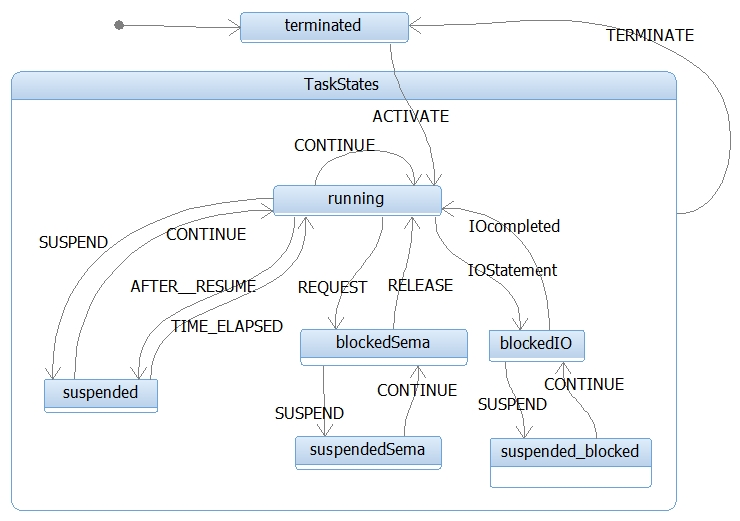
\includegraphics[width=14cm]{taskStatesPEARL.jpg}
\caption{Task statediagram derived from the language report.
The bolt operations are omitted, sice they are identical to the
semaphore operations}
\label{taskStatesPEARL90}
\end{figure}


RTOS-UH used a different model, where termination while an active i/o statement
is delayed until the next end-of-record. 
 

OpenPEARL uses an implementation, which is more close to the language report.
All tasking statements which are executed by the task itself are executed 
obviously synchronously. To guarantee atomistic behavior during a 
tasking operation a mutex is locked at the start of each tasking opoeration and 
unlocked at the end of the operation.
Many operations like error checking are common to all platforms of OpenPEARL.
These operations are treated in the class \texttt{TaskCommon}. The platform specific 
stuff is treated for linux systems and for FreeRTOS based systems.

The suspend and continue operations are difficult to implement with this approach,
since the continue operation must modify the continued task state.
More details are described in chapter \ref{linux_suspend}, \ref{linux_terminate}.

The linux platform uses pthreads for the task realization. The pthreads on linux systems
do not allow to suspend a thread. To realize suspending a task the linux 
implementation of the tasks use a pipe to suspend a thread. 

The linux implementation of \texttt{CONTINUE} must enshure, that the continued task 
updates its task state before other tasks may execute other tasking operation for this task.
Thus in the platform independent part there is a asymetry that the following operations
does not release the lock on the mutex 
\begin{description}
\item [suspend] in case of self suspension
\item [scheduleCallback] in case of self suspension
\item [treatCancelIO] is case of self suspension
\end{description}
It must be regarded by FreeRTOS based implementaion of the tasking operations.


Tasking statements concerning other tasks are a little 
bit more difficult, because the runtime system uses internally semaphore
 and mutex
variables to avoid race conditions on i/o operations.
During such a critical region,
no task termination must occur. So the  {\em remote suspend request} and 
{\em remote termination request} just set a flag and wait for the fulfilling
 of the 
tasking statement from the adressed task. The priority of the 
task to be suspended or terminated is set to the best priority in the system.
Each task has synchronisation points,
which are
\begin{itemize}
\item  after each source statement and
\item  in each synchronisation statement and 
\item in each i/o operation on the system device.
\end{itemize}

During i/o-operation it is a little bit more complicated. OpenPEARL
recommends like stated in the language report that suspend and terminate
effect the task state immediatelly.
In order to interrupt a blocked i/o operation, each platform MUST implement 
methods in the system dation's implementation to SUSPEND and TERMINATE a task while 
performing i/o operations.

The system device driver must invoke a platform dependent method
\verb|treatCancelIO| which will throw ether an exception
(\verb|TerminateRequestSignal|) in case of a termination request
 or just suspends itself.
The TerminateRequestSignal is caught and rethrown at each block which 
locks internal mutexes or semaphores. These variables are unlocked in
the exception handler and the exception is rethrown up to the upmost i/o-API
function.

For the list of specialized tasking methods please refer the
{\em pure virtual} methods of \verb|TaskCommon| in the Doxygen
part of the documentation.

The new state diagram is shown in 
fig. \ref{taskStatesOpenPEARL}.
The transitions from the  states {\em terminatePending} and 
{\em suspendPending}  are triggered from the synchronisation points.

\begin{figure}[bpht]
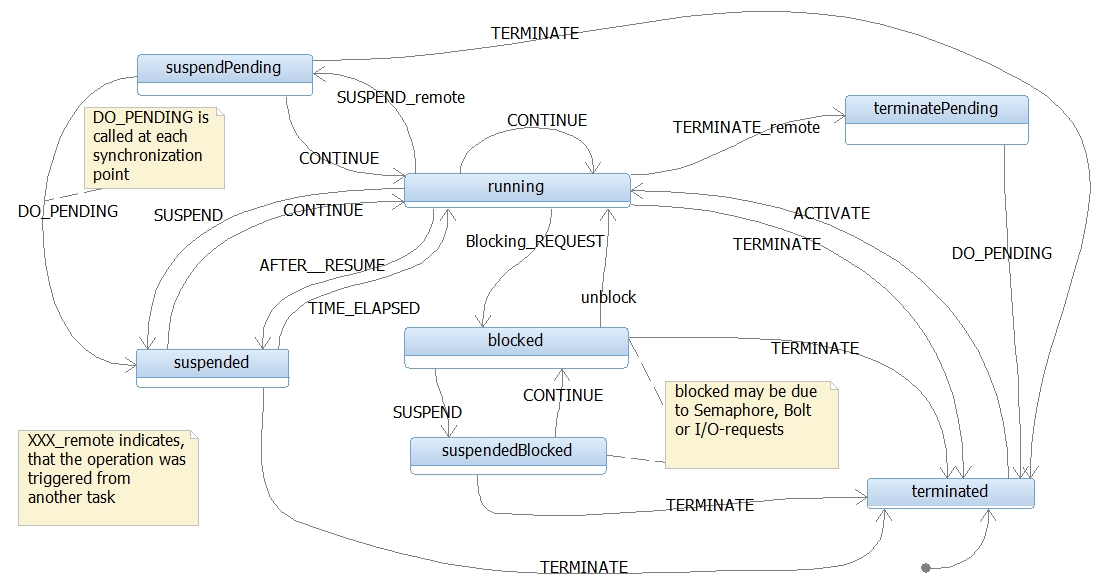
\includegraphics[width=14cm]{taskStatesOpenPEARL.jpg}
\caption{Task statediagram in OpenPEARL.
The states suspendPending and terminatePending were introduced.}
\label{taskStatesOpenPEARL}
\end{figure}
To trigger the events in the state diagram suitable methods in the task 
objects are provided. 

The blocked state is treated differently depending of the block reason, which
is ether:
\begin{description}
\item[REQUEST, ENTER or RESERVE], which means that the task is waiting for 
   the synchronisation variable
\item[IO], which means that the task is currently doing an i/o-operation
   on an user dation
\item[IOWaitQueue], which means that the task is waiting in a priority based
   queue to start it's i/o-operation
\item[IO\_MULT\_IO], which means that the task is waiting in a 
   queue to start it's i/o-operation. The queue is treated by the 
   system dation like in the Console device.
\end{description}

Several classes support the tasking operations:
\begin{description}
\item[class Interrupt] provides the semantics of the PEARL language interrupts
\item[class Semaphore] provides PEARL semaphore semantics with simultanous
   locking on semaphore arrays.
\item[class TaskTimerCommon] provides an interface for the platform
   specific class \verb|TaskTimer|. 
\item[class TaskCommon] provides most of the error checking depending on
   the task state and tasking operation, as well as platform independent
   parts of the tasking operations. Theses operations delegate the concrete
   platform specific operation to the platform specific implementation
   in the class \verb|Task|. The api methods in TaskCommon perform some
    parameter checks and look the mutex for all tasks before delegating 
    the job to the platform specific implementation. 
    The mutex must be unlocked by the target specific implementation 
    after completion of the job. Some operation may need to release and 
    rerequest the mutex in the target specific job --- e.g. suspend,
    which has to block the task until it is continued by another task
    or a scheduded continue.

   Scheduled operations are possible in combination of ACTIVATE, 
   CONTINUE and RESUME.
   The schedule (like AT, ALL, AFTER, WHEN,..) is passed to the 
   tasks methods. The way of treatment (by timers, specific timer threads, ... )
   is decided by the platform code.

   For details about the API of the provided methods, please check the doxygen 
   version of the documentation.
   Please run  the command \verb|make doc| in the base dirtectory of the
   desired platform.

\item[class TaskList] provides a list of all defined PEARL tasks
\item[class TaskMonitor] keeps track of all scheduled and active tasks and
   detects the end of the application.
\item[class Control] allows setting the exit status for the application. 
  The treatment of this status is platform specific.
\end{description}

\section{Thread Safety}
The task state is stored in the task control block, which is realized
by attributes of the \verb|Task|-objects.
The mutual exclusion is realized by  public class methods
\begin{itemize}
\item \verb|TaskCommon::mutexLock()|
\item \verb|TaskCommon::mutexUnlock()|
\end{itemize}
 
This mutex is used in the task related classes, as well as in the interrupt,
semaphore, bolt and i/o related classes. 

All tasking related methods, which check or modify  the tasks state lock the 
mutex variable. Some parts of execution are delegated to platform specific
code. For details about unlocking the mutex please check the code
documentation from doxygen.



\section{Specification and Declaration}
\begin{description}
\item[SPCTASK] makes the forward declararion of the task object.
    The compiler must add the forward declaraction of all tasks
    used in the module before the first declaration, since C++
    variables have a scope from the line of declaration until 
    the end of the block, which contains the declaration.
    The macro has the tasks name as parameter.
\item[DCLTASK] defines the task itself. The DCLTASK macro is followed
    by a block of statements, which define the tasks content.
    The macro has the tasks name, priority and main-attribute as
    parameter. 
    Priority and isMain-attribute are wrapped by the compiler 
    into \verb|Prio|- and \verb|BitString<1>|-type.
\end{description}

The implementation of task handling is platform specific.
Each platform specific implementation need:
\begin{enumerate}
\item  a class {\em Task} which is derived from {\em TaskCommon}.
\item the suitable definition of the \verb|DCLTASK|- and \verb|SPCTASK|-macros
\item the implementation of the tasking methods
\item a mechanism which activates on system start
   all defined tasks containing the isMain-attribute with true. 
   The sequence is defined by the tasks priority. 
   No priority corresponds to the weakest priority.
\item a mechanism which enables a default signal handler for each task
\item a mechanism which enshures the task termination at the end of
   the task body
\end{enumerate}

\paragraph{Notes}\ \\
\begin{itemize}
\item The macros SPCTASK and DCLTASK are currently sufficient only for
    PEARL programs with one module. When multi-module programs
    are supported by the compiler, the GLOBAL-attribute should be 
    passed additionally to both macros.
\end{itemize}

\section{me-Pointer}
The DCLTASK-macro must define an object with the name of the
task with the type {\em Task}.
The macro must enshure that a variable  {\em Task * me;} exists
and points to the tasks object. This pointer is used
by the compiler to trigger tasking operations of the current
task.

This pointer is passed to every procedure as hidden (first) parameter.
By this mean, each procedure may do tasking operations upon the
task, which uses the procedure.
The {\em me}-pointer is defined to be from the base class  {\em TaskCommon}. 
The runtime tasks are derived from this class, so the pointer to the current 
task fits to {\em me}.

\section{Task Priority}
The tasks default priority is defined in the TASK-statement and passed
as second parameter in the DCLTASK-macro.
Scheduling calls may alter the tasks priority. This new priority is valid 
until a new priority is assigne. At restart of the task the default 
priority is used again. Each platform must provide a class \verb|PrioMapper|.

If the concrete target system (like linux) does not support 255 
 application priorities, the method \verb|fromPearl()| must throw
an exception.


\section{Error Tracing}
The error handling of PEARL is done with SIGNALs.
They are very similar to the exceptions in C++ and JAVA. 
The run time systems throws exepctions which are organized in a
hierarchy to catch several exceptions of one kind in one step.
To provide a backtrace to the originating PEARL source line, the compiler 
must add tracing functions.
\begin{CppCode}
Task::setLocation(const char * fileName, int lineNumber);
\end{CppCode}
The method {\em setLocation()} is supplied with the values from
the PEARL source file.

\begin{CppCode}
const char* filename =  "api.prl";
SPCTASK(t1);
SPCTASK(t2);

DCLTASK(t1,10,1) {
   me->setLocation(10,filename);
   pearlrt::Duration d(5.0);
   me->setLocation(11,filename);
   pearlrt::Duration dur;
   me->setLocation(12,filename);
   dur = d*10.0;
   me->setLocation(13,filename);
   printf("5 sec delay\n");
   me->setLocation(14,filename);
   me->resume(pearlrt::Task::AFTER, pearlrt::Clock(),d);
   me->setLocation(15,filename);    
   printf("after 5 sec all 2 sec during 30 sec activate  t2\n");
   printf("    -> 16 activations\n");
   me->setLocation(16,filename);
   t2.activate(me, pearlrt::Prio(30),
               pearlrt::Task::AFTER|pearlrt::Task::DURING|pearlrt::Task::ALL,
               pearlrt::Clock(), d, pearlrt::Duration(2.0), // at, all
               pearlrt::Clock(),d*6.0,0) ;    
}

int t2counter=0;
DCLTASK(t2,20,0) {
   me->setLocation(17,filename);
   printf("t2 started (%d)\n", ++t2counter);
   me->setLocation(18,filename);
   pearlrt::Duration d(10.0);
   me->setLocation(19,filename);
   d = d / (t2counter-2);
}
\end{CppCode}

As result, uncaught SIGNALS would produce an error message like:
\begin{verbatim}
***************************
* Signal "fixed overflow" occured in api.prl at line 19
* Task T2 terminated
***************************
\end{verbatim}

Details about signal-handling is described in the section about signals.


\chapter{Procedures}

\section{Declaration ans Specification}
PEARL procedures are mapped to C++ functions.
They have a hidden first parameter with the pointer to the executing task.
The namespace rules apply as on data values.


\section{REF PROC}
References to procedures are mapped to the template class Ref, which allows
the assignment and derefence operations.

\section{Formal Parameter Types}
Bit and Char-slices need special attention.

\subsection{Call By Value}
In this case an intermediate copy of the actual parameter 
must become created. This may be done by the C++ compiler via the 
normal call by value mechanisme.

\subsection{INV Call By Value}
This must be treated by the compiler. No assignment is allowed to the formal 
parameter, nether passing by reference without INV to other
procedures is allowed.

\subsection{Call By Reference (IDENT)}
All data types except \textbf{BIT} and \textbf{CHAR} types may be 
passed as C++ pointers.

For \textbf{BIT} and \textbf{CHAR} types the actual parameter may be a slice.
Any changes on the formal parameter must affect the current parameter.
To enshure the operation on the same primary data, \textbf{CHAR} and 
\textbf{BIT} values 
must be passed as slice by value. 
Even overlaping slices in the parameter list may be possible.

Slices \textbf{MUST NOT} passed as pointers, since this may cause
side effects when passing the same slice as different parameters.

Example:
\begin{PEARLCode}
DCL bits BIT(16) INIT('ABCD'B4);
DCL hello CHAR(10) INIT('Hello');
...
p: PROC(b1 BIT(4) IDENT, b2 BIT(16) IDENT, c CHAR(2) IDENT);
   b1 := '5'B4;      !! this affects bits.BIT(2:5) !!
   IF b2.BIT(3) THEN !! this must check the modified value !!
      ...
   FIN;

   c := 'x';         !! set the first two characters of the
                     !! actual parameter to 'x '
END;

t: TASK;
   CALL p(bits.BIT(2:5), bits, hello.CHAR(1:2));
END;
\end{PEARLCode}

\begin{CppCode}
...
pearlrt::BitString<16> _bits(0xabcd);
pearlrt::Character<10> _hello("Hello");

void _p(pearlrt::Task * me,
        pearlrt::BitSlice _b1,
        pearlrt::BitSlice _b2,
        pearlrt::CharSlice _c) {

    // modify the bits in the actual parameter (IDENT)
    _b1.setSlice(CONST_BIT4_five);

    // select the bit inside the slice and obtain the bool value
    if ((_b1.
            getSlice(CONST_FIXED_3)->
            mkBitString(pearlrt::BitString<1>*typeInfo)
        ).getBoolean() ) {
       ...
    }
    ...
   _c.getSlice(CONST_FIXED_1,CONST_FIXED_2)->setSlice(CONST_CHAR_1_x);
}

DCLTASK(_t, ...) {
   ...
   _p(me,*pearlrt::BitSlice(_bits).getSlice(2,5),
         pearlrt::BitSlice(_bits),
         pearlrt::CharSlice(_c).getSlice(1)); 
\end{CppCode}

\paragraph{Notes:} 
\begin{enumerate}
\item Bit and char slices are passed by value. The slices point 
internally to the base data value.
\item passing a slice to another procedure by reference (\textbf{IDENT}) 
is possible as complete or subslice.
\item Constants and \textbf{INV} variables are not allowed as actual
 parameters if the formal parameter is not INV (refer \ref{sec_inv_ident}).
\end{enumerate}

\subsection{INV Call By Reference (IDENT)}
\label{sec_inv_ident}
The compiler must check that there is no change of the actual parameter
by assignment or parameter passing.

The invocation with constants is possible. They must become converted 
to a bit- or char slice by the compiler. For other data types, the compiler
must create a constant data element for the given value.

\subsection{REF Types}
\textbf{REF} types may be passed by value as well as by reference 
( \textbf{IDENT}).
The mapping to C++ pointers applies.
This applies also for type \textbf{REF CHAR(}x\textbf{)}
 (e.g. \textbf{REF CHAR(4)});.

\subsubsection{REF CHAR()}
A type \textbf{REF CHAR()} allows a kind of variable string length.
This type realized in the RefChar-class. 

Depending on the actual parameter, diffent actions must be performed 
by the compiler. If the actual parameter is of type:
\begin{description}
\item[CHAR(x):] A temporary RefChar data must be created and passed.
\item[REF CHAR():] The RefChar data object may by passed directly 
   only by value. Passing a REF CHAR() by IDENT may cause inconsistent
   data storage access, if the REF CHAR() is assigned to a procedure
   local CHAR-variable.
\end{description}

\subsubsection{REF INV CHAR()}
Even constants may be passed. In this case, the compiler must create
a temporary RefChar object for any CHAR-values and expressions.

\subsection{Arrays}
Arrays must be passed in two parameters. The array descriptor and the 
array data.


 

\subsection{STRUCT}
The passing of STRUCTs works like simple variables.

\section{Return Value}
The language report forbids \textbf{REF CHAR()} as result type.


\chapter{Interrupt}
An interrupt is an asynchrous event from the outside world.
It is \textbf{NOT} the hardware interrupt of the processor.

\section{Specification and Declaration}
An interrupt is declared in the system part.

Example: Declare the identifier \verb|ctrlc| as the plattform specific
interrupt source \verb|^C|

\begin{verbatim}
ctrlc: UnixSignal(2);
\end{verbatim}

The specification takes place in the problem part:

\begin{verbatim}
SPC ctrlc INTERRUPT;
\end{verbatim}

A specific plattform may support several different interrupt sources.
All concrete interrupt sources must be derived from the parent class
\verb|pearlrt::Interrupt|.


\section{C++ Mapping between System and Problem Part}
The user defined identifier in the system part denotes a specifice interrupt
source. The identifier in the problem part denotes a generalized interrupt.
The compiler should generate a pointer to the generalized interrupt object like
shown in the example below:

\begin{PEARLCode}
SYSTEM;
  ctrlc: UnixSignal(2);
PROBLEM;
   SPC ctrlc INTERRUPT;
\end{PEARLCode}

The user supplied identifier (\verb|ctrlc|) is used as base of derived
identifiers.
\begin{description}
\item[sys\_] prefix denotes the real defined interrupt object 
\item[\_] prefix (as usual for all user supplied idetifiers) denotes the
    pointer to the generalized interrupt object.
\end{description}

\begin{CppCode}
// SYSTEM;
static pearlrt::UnixSignal sys_ctrlc(2);
       pearlrt::Interrupt * _ctrlc = (pearlrt::Interrupt*)&sys_ctrlc;
// PROBLEM;
extern pearlrt::Interrupt * _ctrlc;
\end{CppCode}

\section{Method Mapping}
The interrupt class provides methods for the PEARL language statements
working directly on interrupts.

The translation from PEARL to C++ is generic. 
The interrupt identifier is a pointer to the generalized interrupt object.

\begin{methodMapping}
\verb|ENABLE|  & \verb|enable()| & \\
\verb|DISABLE|  & \verb|disable()|&  \\
\verb|TRIGGER|  & \verb|trigger()| & \\
\end{methodMapping}

Example:

\begin{PEARLCode}
! ctrlc is specified as INTERRUPT;
...
ENABLE ctrlc;
DISABLE ctrlc;
TRIGGER ctrlc;
\end{PEARLCode}

Should translate into:
\begin{CppCode}
_ctrlc->enable();
_ctrlc->disable();
_ctrlc->trigger();
\end{CppCode}

\section{Usage in Task Scheduling}
See chapter \ref{task}


\chapter{Semaphore}
PEARL requires a semaphore implementation with simultaneous locking
mechanism. This is very unfamiliar in small embedded operation systems.
Despite of the fact that Linux would support this feature for semaphores 
thie mechanisme is implemented in the class {\em Semaphore} using one counting semaphore and a mutex. 
Each multitasking operating system provide these two native elements.
The Semaphore-class uses the common interfaces {\em CSemaCommon} and 
{\em MutexCommon}. Both classes need a plattform specific implementation 
with the names {\em CSema} and {\em Mutex}.

A single PEARL semaphore is
just a counter --- and for diagnosic purposes a pointer to the semaphore''s
name.

The semaphore operation request locks the class mutex to avoid race conditions 
with other tasks semaphore operations. In case of all semaphores value are 
larger than 0, they are decremented and the task continued.
In case of at least one requested single semaphore is 0, the task is added
to a wait queue ({\em PriorityQueue}).

On releasing a PEARL semaphore, the wait queue content is checked if a 
task may become continued. The wait queue is searched in order of the tasks 
priority. The single semaphore''s  values are updated as necessary.

To block a task the class must provided the methods {\em block} and 
{\em unblock}.

\section{Declaration}
The declaration of a PEARL semaphore is always done with a preset value.

\begin{PEARLCode}
DCL s0 SEMAPHORE PRESET(0) GLOBAL;
DCL s1 SEMAPHORE PRESET(1);
DCL s2 SEMAPHORE PRESET(2);
\end{PEARLCode}

The class {\em Semaphore} provides a ctor for definition 
of a semaphore variable.
\begin{description}
\item[Semaphore] takes 2 parameters; the semaphore's name and the preset value.
\end{description}

\begin{CppCode}
pearlrt::Semaphore _s0("_s0",0);
static pearlrt::Semaphore _s1("_s1",1);
static pearlrt::Semaphore _s2("_s2",0);
extern pearlrt::Semaphore _s2; // import
\end{CppCode}

\section{Operations}
The class {\em Semaphore} provides the \verb|static| operations 
{\em request()}, {\em release()} and {\em dotry()}\footnote{try is a reserved
keyword in C++}.

PEARL provides the simultaneous locking pattern on semphores.
This leads to the interface of the operations:
\begin{CppCode}
void Semaphore::request(Task *me, int nbrOfSemas, Semaphore **semas);
void Semaphore::release(Task *me, int nbrOfSemas, Semaphore **semas);
int Semaphore::dotry(Task *me, int nbrOfSemas, Semaphore **semas);
\end{CppCode}

\paragraph{Regard that TRY allows only one sempahore in PEARL.}

\section{Sample Usage}

\begin{PEARLCode}
REQUEST s0,s1,s2;
\end{PEARLCode}

\begin{CppCode}
{
   static Semaphore * semas[] = {&s0,&s1,&s2};
   Semaphore::request(me, sizeof(semas[])/sizeof(semas[0]), &semas);
}
\end{CppCode}

The new block allows the reuse of the identifier {\em semas} in multiple
{\em request}, {\em release} and {\em try} operations in the same 
module.
The static storage declaration provides the initialization before run time.
The size calculation should be executed by the C++-compiler.

\chapter{Bolt}
PEARL requires a BOLT implementation with simultaneous locking
mechanism.

A single PEARL BOLT is
a state variable and a counter --- 
and for diagnosic purposes a pointer to the bolt's name.

All public bolt operations lock the class mutex to avoid race conditions 
with other tasks bolt operations.

On freeing or leaving a PEARL bolt variable,
 the wait queue content is checked if a 
task may become continued. The wait queue is searched in order of the tasks 
priority. 

To block a task the class must provided the methods {\em block} and 
{\em unblock}.

\section{Declaration}
The declaration of a PEARL bolt variable is done without preset value..

\begin{PEARLCode}
DCL b0 BOLT GLOBAL;
DCL b1 BOLT;
DCL b2 BOLT;
SPC b3 BOLT;
\end{PEARLCode}

The class {\em Bolt} provides  a ctor for definition 
of a bolt variable.
\begin{description}
\item[pearlrt::Bolt] takes 1 parameter: the bolt's name.
\end{description}

\begin{CppCode}
pearlrt::Bolt _b0("_b0");
static pearlrt::Bolt _b1("_b1");
static pearlrt::Bolt _b2("_b2");
extern pearlrt::Bolt _b3;
\end{CppCode}

\section{Operations}
The class {\em Bolt} provides the \verb|static| operations 
{\em enter()}, {\em leave()}, {\em reserve()} and  {\em free()}.

PEARL provides the simultaneous locking pattern on bolt variables.
This leads to the interface of the operations:
\begin{CppCode}
void Bolt::enter(Task *me, int nbrOfBolts, Bolt **bolts);
void Bolt::leave(Task *me, int nbrOfBolts, Bolt **bolts);
void Bolt::reserve(Task *me, int nbrOfBolts, Bolt **bolts);
void Bolt::free(Task *me, int nbrOfBolts, Bolt **bolts);
\end{CppCode}

\section{Sample Usage}

\begin{PEARLCode}
ENTER b0,b1,b2;
\end{PEARLCode}

\begin{CppCode}
{
   static Bolt * bolts[] = {&b0,&b1,&b2};
   Bolt::enter(me,
               sizeof(bolts[])/sizeof(bolts[0]),
               &bolts);
}
\end{CppCode}

The new block allows the reuse of the identifier {\em bolts} in multiple
{\em enter}, {\em leave}, {\em reserve} and {\em free} operations
 in the same module.
The static storage declaration provides the initialization before run time.
The size calculation should be executed by the C++-compiler.

\section{Error Handling}
If a LEAVE or FREE is executed upon an non ENTERed or RESERVEd
bolt variable the {\em BoltStateSignal} is induced.

\chapter{Devices and I/O}

PEARL distinguishes between system dations and user dations.
%All examples in the language report shown that the statements TAKE and SEND
%operate directly on system dations like a digital i/o.
The operations TAKE, SEND, READ, WRITE, GET and PUT work only on user dations.
User dations are created upon a system dation.

System part and problem part may be compiled separatelly. Therefore 
no information from the system part may be used to compile the problem part.

To avoid matching problems, the compiler produces an XML-file for each 
module with the import and export interface of the module.
The tool IMC (inter module checker) verifies the matching and creates the
C++ code for the system part.


\section{Not Supported Language Elements}
\begin{description}
%\item[TFU] should be ignored by the compiler
%\item[TFU(MAX)] should be ignored by the compiler
\item[FORBACK] is not supported yet, since tape drives are
   difficult to find
\item[R()] remote format must be treated by the compiler
\end{description}

\section{Declarations in System Part}
The compiler checks the elements for proper grammar and passaes the
parsed elements into an XML-file with the same name as the source file.

To provide complete code examples the linux target is used here.
For details of the used system devices please check chapter \ref{x8632devices}.

\begin{PEARLCode}
MODULE (m1);
SYSTEM;
   output: StdStream(1);
PROBLEM;
MODEND;
\end{PEARLCode}

The IMC will respond with a code like:

\begin{CppCode}
static pearlrt::StdStream s_output(1);
       pearlrt::Device * d_output = &s_output;
\end{CppCode};

All devices are derived from {\em Device}.
Devices for basic dations are derived from {\em SystemDationB},
all other devices are derived from {\em SystemDationNB}.
The upcast of the pointer
to the generic {\em Device*} type enables the compiler to generated 
suitable code for the problem part.

The concrete device object is set to {\em static} to avoid namespace polution.
Only the pointer is needed.

\section{Decoration Scheme for Devices}
We need different obejcts, which concern the same user object.
The user objects are prependend with an underscore (\verb|_|).

\begin{description}
\item[d\_...] denotes the upcasted to {\em Device} 
\item[s\_...] denotes the (static defined) real system device object
\item[\_...] without other prefix)denotes the downcasted object in 
     the C++ code of the problem part
\item[dim\_...] denotes the dimension object, which is relate to the 
   user dation
\end{description}

\section{Bus Device Associations}
The update of the language definition introduced {\em BusDeviceAssociations},
which allows to interconnect system part elements.

E.g.
\begin{PEARLCode}
MODULE (m1);
SYSTEM;
   i2c: I2CBus('/dev/i2c-0',100000);  ! access to i2-c
                                      ! interface with 
                                      ! 100kHz bus speed
   temp: LM75('48'B4) --- i2c;        ! one temperatur
                                      ! sensor at
                                      ! the bus i2c
PROBLEM;
   SPC temp DATION SYSTEM BASIC FIXED(15);
MODEND;
\end{PEARLCode}

\begin{CppCode}
// system part only
static pearlrt::I2CBus s_i2c("/dev/i2c-0",100000);

static pearlrt::LM75 s_temp(&s_i2c,0x48);
       pearlrt::Device * d_temp = &s_temp;
\end{CppCode}

Depending to the characteristics of the bus there may be only one client,
or multiple clients. This is specified in the XML-description of the 
device.

The implementation provides two roles:
\begin{itemize}
\item ConnectionProvider, which represents the bus device
\item ConnectionClient, which represents the component on the bus.
\end{itemize}

The classes for clients are derived from \texttt{SystemDationB}.
The classes for providers are be derived from a class which
defines the interface for the connection. 

E.g.:
\begin{description} 
\item[ \texttt{I2CProvider} ] is common to all plattforms
   and defines the communication interface between provider and client
\item[ \texttt{I2CBus}] implements the access to the i2c-bus on a 
   specific plattform
\item[ \texttt{LM75} ] defines a system dation, which is attached to an i2c-bus.
    This element is plattform independent.
\end{description}

\paragraph{Note:} The client has access to the provider by default, since
the provider is passed as first argument in the ctor of the client.
If the provider needs access to the client, the ctor of the client
should register itself at the provider.


\paragraph{Note:} The second parameter in I2CBus is used in microcontroller
   environmants. The linux systems define the transmission speed at
   another location.

\section{Specifications in Problem Part}
The system device is specified in the problem part.
Depending on the class specifier in the {\em SPC}-statement the concete 
dation type is deduced (see tab. \ref{dationTypes}).

\begin{table}[bpht]
\begin{tabular}{l|l|l|l}
  & BASIC & ALPHIC & ALL / type \\
\hline
SYSTEM & SystemDationB & SystemDationNB & SystemDationNB \\
 & DationTS & DationPG & DationRW \\
\hline
\end{tabular}
\caption{Deduced type of the dation object}
\label{dationTypes}
\end{table}


\begin{PEARLCode}
SPC output DATION OUT SYSTEM ALPHIC GLOBAL;
SPC disc DATION OUT SYSTEM ALL GLOBAL;
SPC console DATION OUT ALPHIC GLOBAL;
SPC logbook DATION OUT Fixed(15) GLOBAL;
SPC mot DATION OUT SYSTEM BASIC BIT(4) GLOBAL;
\end{PEARLCode}

\begin{CppCode}
extern pearlrt::Device * d_output;
static pearlrt::SystemDationNB _output* = 
             static_cast<pearlrt::SystemDationNB*>(d_output);

extern pearlrt::Device * d_disc;
static pearlrt::SystemDationNB _disc* = 
             static_cast<pearlrt::SystemDationNB*>(d_disc);

extern pearlrt::DationPG _console;

extern pearlrt::DationRW _logbook;

extern pearlrt::Device * d_mot;
static pearlrt::SystemDationB * _mot = 
             static_cast<pearlrt::SystemDationB*>(d_mot);
\end{CppCode}

\section{Declaration of a User Dation}
The declaration of user dation may appear inside and outside of procedures and 
tasks.
The declaration leads to an instantiation of an object. 
The class attribute of the user dation decide about the type of the object
(see tab. \ref{dationTypes}).

The different types of possible dimension specifications are mapped to
a class hierarchy for {\em DationDim}s. For details see the doxygen part 
of the runtime documentation.

\begin{PEARLCode}
DCL console DATION OUT ALPHIC DIM(*,80) FORWARD STREAM NOCYCL CREATED(output);
DCL file DATION OUT FIXED(15) DIM(*,80) FORWARD STREAM NOCYCL CREATED(output);
DCL file1 DATION OUT ALL DIM(*) FORWARD STREAM NOCYCL CREATED(output);
DCL motor DATION OUT BASIC BIT(4) CREATED(mot);
\end{PEARLCode}

\begin{CppCode} 
// 2-dimensions, first dimension is unbound
static pearlrt::DationDim2 dim_console(80);
static pearlrt::DationPG _console(_output, 
                pearlrt::Dation::OUT      |
                pearlrt::Dation::FORWARD  | 
                pearlrt::Dation::STREAM   |
                pearlrt::Dation::NOCYCL,
                &dim_console);

static pearlrt::DationDim2 dim_file(80);
static pearlrt::DationPG _file(_output, 
                pearlrt::Dation::OUT      |
                pearlrt::Dation::FORWARD  | 
                pearlrt::Dation::STREAM   |
                pearlrt::Dation::NOCYCL,
                &dim_file, sizeof(pearlrt::Fixed<15>));

static pearlrt::DationDim1 dim_file1();
static pearlrt::DationPG _file1(_output, 
                pearlrt::Dation::OUT      |
                pearlrt::Dation::FORWARD  | 
                pearlrt::Dation::STREAM   |
                pearlrt::Dation::NOCYCL,
                &dim_file, 1);

static pearlrt::DationTS _motor(_mot,
                pearlrt::Dation::OUT);
\end{CppCode}

Remarks:
\begin{itemize}
\item the dation parameters are \verb|or|ed together
\item the dimenion object is defined statically.
\item the {\em CREATED()} parameter is passsed as first parameter
\item if the dation is defined as {\em GLOBAL} the \verb|static| must
  be omitted
\item a user dation with transfer type ALL must be 1-dimensional --- may
be bounded --- and the size of a data element must be specified as 1
\item the userdations of type BASIC do not allow Topology- and 
AccessAttribut-specifications 
\end{itemize}

\subsection{DIRECT Dation}
DIRECT dations are implemented on e.g. disc files
\begin{itemize}
\item    as artificial array like structure
\item    the DIM-specifies the structure
\item    absolute positioning is allowed
\item    relative positioning is mapped on the absolute positioning
\item    STREAM allows the positioning across dimension limits
\item    STREAM allows silent reading and writing across dimension limits
 \item   CYCLIC realizes a cyclic positioning modulo the complete
        dimension in both directions
\item    CYCLIC realizes a cyclic writing in that way that a
          repositioning to the beginning of the dation is inserted
          at the end of the dation, if the system device does not support
          CYCLIC operation with the same dimension
%\item    unwritten locations in the dations contain undefined values
\item    CYCLIC on unbounded dations is ridiculous
\end{itemize}

\subsection{FORWARD Dation}
FORWARD and CYCLIC is ridiculous if the system dation is not CYCLIC,
 since FORWARD can not rewind.

FORWARD dations are typically used on devices like stdin, 
stdout or TCP/IP-sockets.

\begin{description}
\item[PUT/GET] dations are created on e.g. stdout. 
   \begin{itemize}
   \item PUT ... BY X, SKIP and PAGE write space, new line or formfeeds
         as required by format
   \item  GET ... BY X, SKIP and PAGE discard input characters until the
         required number of characters, newlines or formfeeds were detected
   \item NOSTREAM causes 
        the specified dimension is used for error detection. 
         GET/PUT across boundary cause an error condition
   \item STREAM:
         number of dimensions control the possibility for X,SKIP and PAGE
         no boundary enforced
   \end{itemize}

\item[READ/WRITE] positioning:
   \begin{itemize}
     \item WRITE ... BY  X,SKIP and PAGE fills zero-records as required 
           by the current location
     \item READ ... BY  X,SKIP and PAGE discards input until 
           the required location is reached.
   \end{itemize}
\item[READ/WRITE + NOSTREAM] dations are implemented on e.g.
        TCP/IP socket or pipes
   \begin{itemize}
    \item The specified dimension is used for error detection
    \end{itemize}
\item[ READ/WRITE + STREAM] will  
        normalize the current location to be within the specified dimensions
        by calculating any out of bounds position by simulating line
        and page wraps. Eg:
\begin{verbatim}
DIM( 10,80)
! current location: (5,79)
WRITE a,b,c TO ...; --> new logical location (5, 81)
WRITE d TO .. BY SKIP;
\end{verbatim}
    \begin{itemize}
     \item calculate virtual normalized location: (6,1)
     \item SKIP fills 79 records with 0; new location (7,1)
     \item d will be written on location (7,1); new location is  (7,2)
     \end{itemize}
\end{description}

\subsection{TFU}
TFU requires an input/output buffer for the data.
The size of this buffer is definied by the record size from the DIM-attribute
and the data size.

The general behavior of a dation in context of usage from different tasks 
is not affected. 
The only problem occurs with the console device, which allows more than one 
operation to be pending from different tasks. In order to avoid race conditions
the SystemDationNB interface contains the method 
\texttt{informIOOperationComplete} , which triggers the next pending output 
operation in the system dation \texttt{Console}.

\section{Concurrency during I/O}
\label{ioconcurrency}

\subsection{Concurrency on the same user dation}
It is never stated but clearly appreciated that i/o-statements from
different tasks should not intermix within their i/o-operations.
This behavior is achieved by the {\em beginSequence} and 
{\em endSequence} clause. 
This clause  checkes if a user dation is currently busy or not.
If the user dation is busy, the i/o request is placed in a priority
based waitqueue. In {\em endSequence} the wait queue is checked for
pendings requests.

In case of abnormal termination due to signals in the try-block
the {\em endSequence} in the catch-clause releases the used mutex.
If a RST-value is specified in the statement the given variable is
updated, else the exception is rethrown.

In case of invocation a \textbf{TERMINATE} on a task beeing busy in i/o,
the device driver is informed to abort the i/o request and emit the
{\em TerminateIOSignal}, which is caught in each superior layer 
in the i/o stack which needs postprocessing in this case.


\begin{PEARLCode}
DCL (x,y) Fixed(15);
DCL rst Fixed(31);
...
PUT x,y TO console BY F(4), RST(rst), F(5), SKIP;
\end{PEARLCode}

\begin{CppCode}
Fixed<31> rst;
Fixed<15> x
Fixed<15> y;

{
   // setup data list and format list

   // the blocking was moved into the user dation
   // operations put(), get(), ...
   _console.put(me, dataList, formatList);
}
\end{CppCode}

Inside the put,get,read,write, take and send methods a
try-catch-clause captures all PEARL-signals from the code in the 
type block. If a RST-value is specified in the format list, the method
{\em updateRst} will assign the actual signal code to the RST-variable.
If no RST-vale is specified for this statement, the signal is propagated.
If the error is produced in the formatting of x, a signal is thrown.
If the error is produced in the formatting of y, no signal is thrown but rst
is set.

If the system dation supports multiple io-operations in the same time,
the locking mechanism of the user dation is switched off, by implementing
a method \verb|bool allowMultipleIOOperations()| in the system dation.
In this case, ths system dation is responsible for proper operation.

\subsection{Concurrency on the same system dation}
It is possible to create several user dations upon the same system dation.
If the operation on the system dation is not reentrant, the developer must
enshure by additional mutex variables, that those operations do not operlap.

\section{Open and Close}
The super class UserDation knows the OPEN and CLOSE operations.
Both have optional parameters. This is solved by a \verb|or|ed
parameter.

\begin{PEARLCode}
DCL f FIXED(31);
...
OPEN console;
...
OPEN logbook BY RST(f), IDF('file.001') ANY;
...
CLOSE console;
...
CLOSE logbook BY CAN;
\end{PEARLCode}

\begin{CppCode}
Fixed<15> f;
...
_console.dationOpen();
...
{
   static Character<8> fileName("file.001");
   _logbook.dationOpen(Dation::IDF|Dation::ANY| Dation::RST, &fileName ,& f);
}
...
_console.dationClose();
...
_logbook.dationClose(Dation::CAN);
\end{CppCode}

Remarks:
\begin{itemize}
\item The presence of a rst-value is signaled by the \verb|or|ed parameter
   in dationOpen and dationClose
\item The filename must be passed by reference. The corresponding
   object must be defined. Eg. as \verb|static| is a new block.
\item The runtime system checks whether the dation parameters from
   user dation match the system dation's parameters. 
   If they do not match a PEARL signal is raised
\end{itemize}

\section{System Dation API}
The API consists of of usual methods
\begin{itemize}
\item dationOpen
\item dationClose
\item dationRead
\item dationWrite
\end{itemize}

Addionally the following methods must be provided
\begin{description}
\item[capabilities] must return a bit map about the supported 
   capabilities like FORWARD, DIRECT, IN, OUT, CAN,... of the system dation
\item[suspend] must suspend the i/o operation. No further i/o operation 
must be performed  until the task becomes continued or terminated.
\item[terminate] must cancel the i/o operation and emit the 
\verb|IOTerminationRequestSignal|, which is caught in superior levels
 of the i/o stack in order to free any allocated semaphorfes or mutexes.
\end{description}

The details of the API are documented in the doxygen part of the documentations.


\section{IO Transfer Operations}
The IO-operations are treated by methods  of the user dations.
These methods receive a list of data elements and a list of format
elements. These lists will be treated according the semantics of the dation
type. ALPHIC dation are controlled by the data list and will use
the format list cyclic, if more data than formats are in the list.
Non basic dations with a specific data type will treat all positioning
elements first followed by the treatment of the data elements. 
The locking mechanisme \ref{ioconcurrency} is realized inside of these methods.

For details see the source code documentation of the classes
\begin{description}
\item[IODataEntry] the individual data entries
\item[IODataList] the list of all data entries for one statement
\item[IOFormatEntry] the individual format entries
\item[IOFormatList] the list of all format entries for one statement
\end{description}

All parameters of format elements are expected as type
\verb|pearlrt::Fixed<31>|.

The effective code will be in this case:
\begin{CppCode}
Fixed<31> rst;
Fixed<15> x
Fixed<15> y;

{
  // setup io data and format lists in a new block
  // define variables for expression results in data list and format list
  ...
  IODataEntry dataEntries[] = { {...},{...},...};
  IODataList dataList = {sizeof( dataEntries)/sizeof(dataEntries[0]),
                         dataEntries};
  IOFormatEntry formatEntries[] = { {...},{...},...};
  IOFormatList formatList = {sizeof( formatEntries)/sizeof(formatEntries[0]),
                         formatEntries};
  // evaluate expressions in datalist and format list
  _console.put(me, dataList, formatList);
  // leave block with put statement
}
\end{CppCode}

\subsection{Structs}
Struct components must be rolled out for CONVERT, PUT and GET.

\subsection{Array of Structs}
An array of struct is passed to the io-system as a loop with the 
rolled out pointers for the first loop iteration.
The loop parameters are:
\begin{description}
\item[dataType.width] contains the number of items in this loop
\item[dataPtr.offsetIncrement] contains the size of the struct
\item[param1.numberOfElements] is a pointer to the number of array
    elements 
\end{description}

If a struct contains another array of struct as a compontent, this
structure is nested up to 11 levels.


\subsection{Array slices}
Arrays and array slices of simple types are passed to the i/o system
as
\begin{description}
\item[.dataPtr] pointer to the first data element
\item[.param1.numberOfElements] pointer to the number of elements.
     This may be ether a pointer to a constant,
      or a pointer to temporary variable, if a limits are
      calculated at run time.
\end {description}

\subsection{BIT Slices}
Bit slices are not possible as struct component and as arrays.
They are passed as 
\begin{itemize}
\item pointer and size of the parent bit string
\item pointer to the starting bit number (\texttt{size\_t*}) 
\item pointer to the last bit number (\texttt{size\_t*})
\end{itemize}

For details check the source code documentation of the file \texttt{IOJob.h}



\chapter{Linux specific Part}
\import{../linux/doc/}{os.tex}
\import{../linux/doc/}{tasking.tex}

\chapter{Common Part for FreeRTOS based Microcontroller Systems}
\import{../FreeRTOS/doc/}{basics.tex}

\chapter{LPC1768: ARM Cortex M3 (Landtiger) specific Part}
\import{../lpc1768/doc/}{os.tex}
\import{../lpc1768/doc/}{system.tex}
\import{../lpc1768/doc/}{devices.tex}
\import{../lpc1768/doc/}{technicaldata.tex}

\chapter{ESP32: Xtensa Dual Core Processor}
\import{../esp32/doc/}{buildsystem.tex}

\chapter{Add new Platform}
\section{Basic about the Build System}
The build system is based in make.
At top level of OpenPEARL the configuration is set using Kconfig.

If a new platform should be added some changes must be done to integrate
the new platform to the OpenPEARL build system.

\paragraph{Note:}
Be aware that OpenPEARL is provided under a 3-clause BSD license.
Do not integrate any parts which violates this license.

\begin{enumerate}
\item Invent a suitable identifier for the new platform
like \verb|esp32|.
\item define a numeric id for the platform like 3. This number is required
  to select a specific platform for the application build.
  Refer to the used numbers in the target 'install' 
  in \verb|runtime/Makefile|.
\item define a preprocessor identifier for small platform specific
   changes in common files for similar platforms, like \verb|OPENPEARL_ESP32|.
   Pass this identifier with the \verb|-D| option to the c/c++ compiler
\end{enumerate}

\section{Kconfig}
Add in \verb|configuration/fm| a platform specific Kconfig file and add this 
file to \verb|configuration/fm/runtime.fm|.

\begin{itemize}
\item provide an overall option \verb|XXX| 
   to enable the platform and set the default 
      to 'n'
\item provide additional options required and set then as 
   \verb|depends on XXX|
\end{itemize}

\section{Integration to the Build system}
\begin{itemize}
\item create a directory for your platform in \verb|.../runtime/| (eg. esp32)
\item provide a \verb|Makefile| in the platform directory for the
   targets
  \begin{description}
  \item[clean] as usual 
  \item[all] just build the platform specific files. Additionally,
     the build system expects
     \begin{description}
        \item[pearl.h] with a single header file for this platform with 
         all OpenPEARL specific classes. You create this with the 
         \em{include composer}
       \item[cc\_bin.inc] must invoke the compiler with all required 
                flags. Use \verb|$fn.cc| for the name of the application
                source file and \verb|system.cc| for the representation
                of the system part.
       \item[run\_bin.inc] do all operations to start the application on
               your platform. This includes specific file translations and
               downloading.
     \end{description}
  \item[install] copy the platform specific files to 
	\verb|$CONFIG\_INSTALL\_Target|
  \item[prepare] create dummy files for the files to be installed later.
    And set rw-permisions for regular users. This build is executed 
    initially with root-priviledges
  \end{description}
\item add your platform to \verb|runtime/Makefile| in the make targets
   \begin{itemize}
   \item prepare
   \item install
   \item cc\_bin.inc
   \item run\_bin.inc
   \item and a plain target for your platform, which invokes for the target
      'all' (eg. esp32)
   \end{itemize}
\item if you need special OpenPEARL signals in your platform, refer to the 
   chapter \ref{sec_signal_definition}.
\item provide a platform manual, which describes the usage of the new platform.
\end{itemize}



\chapter{List of all Signals}
\import{../common/}{signallist.tex}

\begin{thebibliography}{99}
\bibitem{mueller2016}  
   M.Schaible, R. M\"uller; Konsistenzpr\"ufungen in OpenPEARL,
   In W.A. Halang, H. Unger (Hrsg.): Informatik aktuell --- 
   Internet der Dinge und Echtzeit, Springer Verlag, 2016

\bibitem{msc_hertwig}
    Stephan Hertwig: SmallPEARL ---
    Treiber f\"ur die Peripherieinfrastruktur des Raspberry,
    Masterthesis FernUNI Hagen, Sommerseemster 2015
 
\bibitem{openpearlss16}
    M.Bauer, T.Schaz, J.Weber, T. Welte, J. Wirth: OpenPEARL,
    Projektarbeit im Studiengang AIB/CNB der HS Furtwangen, Sommersemester 2016

\bibitem{runtime}
   R. M\"uller: OpenPEARL - Runtime System, Project Document

\bibitem{msc_beyer}
   M. Beyer: ????,
   Masterthesis HS Furtwangen, Sommersemester 2018

\end{thebibliography}
~                          


\end{document}

